
\documentclass[10pt]{sigplanconf}

% Packages LaTeX
% Packages.tex

% Packages di latex utilizzati 

  % Standard dell'ams
\usepackage{amssymb,amsmath}

  % Per le definizioni di connessioni di Galois
\usepackage{galois}

  % Per formattare ed includere il testo
\usepackage{lgrind}
     % Cambiamento dei font per lgrind: tutti in Courier
\def\CMfont{\ttfamily\itshape}
\def\KWfont{\ttfamily\bfseries}
\def\VRfont{\ttfamily}
\def\BGfont{\ttfamily}
\def\NOfont{\ttfamily}

  % Caratteri speciali per i nomi di funzione
\usepackage{bbm}

  % Caratteri ``cal'' carini
\usepackage[mathcal]{euscript}

  % per \baro
\usepackage{stmaryrd}

  % per \xspace
\usepackage{xspace}

  % per i diagrammi
\usepackage[all]{xy}

  % for scalebox
\usepackage{graphicx}
 
   % Per le figure incastrate l'una nell'altra
\usepackage{subfigure}

  % Per le figure nel testo
\usepackage{wrapfig}


\usepackage{tabularx}

  % Per includere i verbatim
\newbox\subfigbox
\makeatletter
\newenvironment{subfloat}
{\def\caption##1{\gdef\subcapsave{\relax##1}}%
\let\subcapsave\@empty
\setbox\subfigbox\hbox
\bgroup}
{\egroup
\subfigure[\subcapsave]{\box\subfigbox}}
\makeatother

   % Per la compilazione Condizionale
\usepackage{ifthen}

\usepackage{empheq}

   % Per i riferimenti incrociati



%\ifx\pdfoutput\undefined % Se compilo con ``latex'' ed uso ps2pdf
%\usepackage{color}
%\usepackage[dvips]{graphicx}       %%% graphics for dvips
%\DeclareGraphicsExtensions{.eps}   %%% standard extension for included graphics
%\usepackage[bookmarks=true]{hyperref}
%\else                    % Se compilo con ``pdflatex'' 
%\usepackage[pdftex]{graphicx}      %%% graphics for pdfLaTeX 
%\DeclareGraphicsExtensions{.pdf}   %%% standard extension for included graphics
%\usepackage[pdftex]{thumbpdf}      %%% thumbnails for pdflatex
%\usepackage[pdftex,                %%% hyper-references for pdflatex
%bookmarks=true,%                   %%% generate bookmarks ...
%bookmarksnumbered=true,%           %%% ... with numbers
%hypertexnames=false,%              %%% needed for correct links to figures !!!
%breaklinks=true,%                  %%% break links if exceeding a single line
%linkbordercolor={0 0 1}]{hyperref} %%% blue frames around links
%                                  %%% pdfborder={0 0 1} is the default
%\hypersetup{
%pdfauthor   = {Francesco Logozzo \& Agostino Cortesi},
%pdftitle    = {to be decided},
%pdfsubject  = {Objects},
%pdfkeywords = {Abstract Interpretation, Static Analysis, Object Oriented}
%}
%\pdfadjustspacing=1                %%% force LaTeX-like character spacing
%\fi 


%%% Local Variables: 
%%% mode: plain-tex
%%% TeX-master: "main"
%%% End: 


% Definizioni di Macro ed ambienti
% Definizione dei simboli

\newcommand{\eg}{\textit{e.g.}}
\newcommand{\ie}{\textit{i.e.}}

% Definizione dell' operatore di astrazione
\newcommand{\abs}[1]{\ensuremath{\bar{\mathsf{#1}}}}

\newcommand{\sx}{\llbracket}
\newcommand{\dx}{\rrbracket}

  % Semantica generica
\newcommand{\sem}[1]{\ensuremath{\sx \mathtt{#1} \dx}}

  % Semantica che prende un nome
\newcommand{\semantica}[2]{\ensuremath{\mathbb{#1}\sem{#2}}}

\newcommand{\BigSemantica}[2]{\ensuremath{\mathbb{#1}{\Bigg\llbracket #2 \Bigg\rrbracket}}}

  % Semantiche generiche
\newcommand{\csem}[1]{\ensuremath{\semantica{s}{#1}}}
\newcommand{\asem}[1]{\ensuremath{\semantica{\abs{s}}{#1}}}
\newcommand{\asemRefined}[1]{\ensuremath{\semantica{\abs{s}^*}{#1}}}

  % Funzione di ``transfer''
\newcommand{\trasf}[1]{\ensuremath{\semantica{t}{#1}}}
\newcommand{\atrasf}[1]{\ensuremath{\semantica{\abs{t}}{#1}}}

  % Semantica di: costruttore,  metodo
\newcommand{\semcostr}[1]{\semantica{i}{#1}}
\newcommand{\semmetodo}[1]{\semantica{m}{#1}}
\newcommand{\semoggetto}[1]{\semantica{o}{#1}}
\newcommand{\semclasse}[1]{\semantica{c}{#1}}

  % Semantica Colleting Traces
\newcommand{\Semmetodo}[1]{\semantica{M}{#1}}
\newcommand{\Semoggetto}[1]{\semantica{O}{#1}}
\newcommand{\Semclasse}[1]{\semantica{C}{#1}}

  % Semantics Reachable States
\newcommand{\rsemcostr}[1]{\semantica{I}{#1}}
\newcommand{\rsemmetodo}[1]{\Semmetodo{#1}}
\newcommand{\rsemoggetto}[1]{\semantica{O}{#1}}
\newcommand{\rsemclasse}[1]{\semantica{C}{#1}}

  % Seamntica Astratta
\newcommand{\asemcostr}[1]{\semantica{\bar{I}}{#1}}
\newcommand{\asemmetodo}[1]{\semantica{\bar{M}}{#1}}
\newcommand{\asemoggetto}[1]{\semantica{\bar{O}}{#1}}
\newcommand{\asemclasse}[1]{\semantica{\bar{C}}{#1}}

  % Operazioni su stati
\newcommand{\less}{\ensuremath{\sqsubseteq}}
\newcommand{\join}{\ensuremath{\sqcup}}
\newcommand{\meet}{\ensuremath{\sqcap}}
\newcommand{\bottom}{\ensuremath{\bot}}
\newcommand{\bigjoin}{\ensuremath{\bigsqcup}}

  % Semantica astratta
\newcommand{\asemantica}[2]{\semantica{\bar{#1}}{#2}}
\newcommand{\asemanticaBig}[2]{\BigSemantica{\bar{#1}}{#2}}


  % Semantica astratta BIS, per aggiungere pedici
\newcommand{\asemanticaBis}[3]{\semantica{\bar{#1}_{\textit{#2}}}{#3}}

  % Operazioni astratte
\newcommand{\nabs}[1]{\bar{#1}}
\newcommand{\abot}{\nabs{\bot}}
\newcommand{\atp}{\nabs{\ensuremath{\top}}}
\newcommand{\aless}{\nabs{\less}}
\newcommand{\asup}{\ensuremath{\nabs{\sqsupseteq}}}
\newcommand{\acup}{\ensuremath{\nabs{\sqcup}}}
\newcommand{\ajoin}{\acup}
\newcommand{\abigcup}[1]{\nabs{\bigsqcup_{#1}}}
\newcommand{\abigjoin}[1]{\abigcup{#1}}
\newcommand{\acap}{\ensuremath{\nabs{\sqcap}}}
\newcommand{\ameet}{\acap}
\newcommand{\abigcap}[1]{\nabs{\bigsqcap_{#1}}}
\newcommand{\abigmeet}[1]{\abigcap{#1}}


 % lfp : least fixpoint
\newcommand{\lfp}[2]{\ensuremath{\mathrm{lfp}^{#1}_{#2}}}

 % gfp: greatest fixpoint
\newcommand{\gfp}[2]{\ensuremath{\mathrm{gfp}^{#1}_{#2}}}


% Insiemi e Funzioni

  % Insieme, elemento di insieme, nessun elemento
\newcommand{\insieme}[1]{\ensuremath{\mathsf{#1}}}
\newcommand{\el}[1]{\ensuremath{\mathsf{#1}}}
\newcommand{\noel}{\el{\bot}}

  % Insieme delle parti
\newcommand{\parti}[1]{\ensuremath{\mathcal{P}{(#1)}}}
\newcommand{\partiFin}[1]{\ensuremath{\mathcal{P}_{\mathrm{fin}}{(#1)}}}


  % Elementi di insiemi
\newcommand{\noval}{\ensuremath{\baro}}

  % Cardinalita di inisiemi
\newcommand{\cardinalita}[1]{\ensuremath{\# #1}}

  % Env, Store, Addr, Val, Label : Scorciatoie
\newcommand{\env}{\insieme{Env}}
\newcommand{\Env}{\env}

\newcommand{\aenv}{\ensuremath{\bar{\env}}}

\newcommand{\store}{\insieme{Store}}
\newcommand{\Store}{\store}

\newcommand{\astore}{\ensuremath{\overline{\store}}}

\newcommand{\AState}{\abs{\Sigma}}
\newcommand{\astate}{\AState}

\newcommand{\addr}{\insieme{Addr}}
\newcommand{\Addr}{\addr}

\newcommand{\aaddr}{\ensuremath{\overline{\addr}}}

\newcommand{\Reference}{\insieme{Ref}}
\newcommand{\reference}{\reference}

\newcommand{\AReference}{\ensuremath{\overline{\Reference}}}

\newcommand{\val}{\insieme{Val}}

\newcommand{\etichetta}{\insieme{Label}}
\newcommand{\cont}{\ensuremath{\kappa}}

  % Stati
\newcommand{\stati}[1]{\ensuremath{\Sigma}}
  % Tracce
\newcommand{\tracce}[1]{\ensuremath{\mathcal{T}(#1)}}
  % Transizione
\newcommand{\tr}[1]{\ensuremath{\xrightarrow{#1}}}

  % Insieme di funzioni
\newcommand{\funzione}[2]{\ensuremath{[#1 \rightarrow#2]}}

  % Funzione vuota
\newcommand{\emptyfun}{\ensuremath{[\cdot]}}

  % Insieme di funzioni monotone e joim-morphism
\newcommand{\funmon}[2]{\ensuremath{[#1 \stackrel{m}{\longrightarrow} #2]}}
\newcommand{\funjoin}[2]{\ensuremath{[#1 \stackrel{\sqcap}{\longrightarrow} #2]}}

% Astratto
  % Dominio concreto
\newcommand{\dom}[1]{\insieme{#1}}

  % Dominio astratto
\newcommand{\adom}[1]{\ensuremath{{\mathsf{#1}}}}

 % Vari domini
\newcommand{\Intervals}{\dom{Intv}}
\newcommand{\LT}{\dom{LT}}
\newcommand{\Boxes}{\dom{Boxes}}
\newcommand{\DBM}{\dom{DBM}}
\newcommand{\Octagons}{\dom{Oct}}
\newcommand{\Polyhedra}{\dom{Poly}}
\newcommand{\Poly}{\Polyhedra}
\newcommand{\Lineq}{\dom{LinEq}}
\newcommand{\LinEq}{\Lineq}
\newcommand{\Karr}{\Lineq}
\newcommand{\Symbolic}{\dom{Symb}}
\newcommand{\Pentagons}{\dom{Pnt}}
\newcommand{\SubPolyhedra}{\dom{SubPoly}}
\newcommand{\SubPoly}{\SubPolyhedra}
\newcommand{\Subpoly}{\SubPolyhedra}

  % Elemento di dominio astratto
\newcommand{\ael}[1]{\ensuremath{\abs{\el{#1}}}}
\newcommand{\aelBis}[2]{\ensuremath{\abs{\el{#1}}_\el{#2}}}

  % Funzione di astrazione e concretizzazione
\newcommand{\alfa}{\ensuremath{\alpha}}
%\renewcommand{\gamma}{\ensuremath{\gamma}}
\newcommand{\gm}{\ensuremath{\gamma}}


% Funzioni usate nella tesi
  % Transizione basica
\newcommand{\prossimo}{\ensuremath{\mathrm{next}}}
%\newcommand{\next}{\ensuremath{\mathrm{next}}}
\newcommand{\nextDir}{\ensuremath{\mathrm{next_{dir}}}}
\newcommand{\nextInd}{\ensuremath{\mathrm{next_{ind}}}}
\newcommand{\prossimoDir}{\nextDir}
\newcommand{\prossimoInd}{\nextInd}

  % Transizione ``collecting''
\newcommand{\Next}{\ensuremath{\mathrm{Next}}}
\newcommand{\NextDir}{\ensuremath{\mathrm{Next_{dir}}}}
\newcommand{\NextInd}{\ensuremath{\mathrm{Next_{ind}}}}

  % Reachable addresses
\newcommand{\reachable}{\ensuremath{\mathrm{reachable}}}
  % Update function
\newcommand{\update}{\ensuremath{\mathrm{update}}}
  % Storia delle interazioni
%\newcommand{\etichette}{\ensuremath{\mathrm{labels}}}
\newcommand{\storia}{\ensuremath{\mathrm{history}}}

  % Contesto
\newcommand{\contesto}{\ensuremath{\mathrm{Context}}}

  % Contesto Astratto
\newcommand{\acontesto}{\ensuremath{\mathrm{\overline{Context}}}}

% Tracce : definizioni
\newcommand{\stringavuota}{\ensuremath{\epsilon}}


% Funzioni di astrazione
  % Prima Astrazione, quella dei metodi
\newcommand{\alfaPrima}{\ensuremath{\alpha_{\Yright}}}
\newcommand{\gammaPrima}{\ensuremath{\gamma_{\Yright}}}
  % Versione higher-order
\newcommand{\alfaPrimaDot}{\ensuremath{\dot{\alpha}_{\Yright}}}

  % Seconda Astrazione, quella degli stati
\newcommand{\alfaSeconda}{\ensuremath{\alpha_{\circ}}}
\newcommand{\gammaSeconda}{\ensuremath{\gamma_{\circ}}}
  % Versione higher-order
\newcommand{\alfaSecondaDot}{\ensuremath{\dot{\alpha}_{\circ}}}


\newcommand{\alfaAddr}{\ensuremath{\alpha_\el{a}}}
\newcommand{\gammaAddr}{\ensuremath{\gamma_\el{a}}}

\newcommand{\gammaBool}{\ensuremath{\gamma_\el{b}}}

\newcommand{\gammaEnv}{\ensuremath{\gamma_\el{e}}}

\newcommand{\gammaOct}{\ensuremath{\gamma_\el{o}}}
\newcommand{\gammaDOct}{\ensuremath{\gamma_\el{do}}}

\newcommand{\gammaRef}{\ensuremath{\gamma_\el{r}}}

\newcommand{\gammaStore}{\ensuremath{\gamma_\el{s}}}

\newcommand{\gammaState}{\ensuremath{\gamma_{\astate}}}

% Estensioni per OO

  % Classe
\newcommand{\classe}[1]{\ensuremath{\mathtt{#1}}}
\newcommand{\classi}{\ensuremath{\mathcal{C}}}

  % Gerarchia
\newcommand{\gerarchia}[1]{\ensuremath{\mathcal{#1}}}
\newcommand{\gerarchie}{\ensuremath{\mathbb{H}}}

  % Operatori su Gerarchie 
\newcommand{\inserisciClasse}{\ensuremath{\uplus}}
\newcommand{\costruisciClasse}{\ensuremath{\beta}}
\newcommand{\unisciGerarchie}{\ensuremath{\Cup}}

\newcommand{\aclasse}[1]{\ensuremath{\abs{\mathtt{#1}}}}
\newcommand{\aclasseLong}[1]{\ensuremath{\overline{\mathtt{#1}}}}
  % Oggetto, instanza di classe
\newcommand{\oggetto}[1]{\ensuremath{\mathsf{#1}}}
  % Metodo
\newcommand{\metodo}[1]{\ensuremath{\mathtt{#1}}}
  % Campo
\newcommand{\campo}[1]{\ensuremath{\mathtt{#1}}}

  % Astrazioni di campi
\newcommand{\acampo}[1]{\ensuremath{\mathtt{\abs{#1}}}}

  % Astrazione di metodi con constraints
\newcommand{\ametodo}[1]{\ensuremath{\mathtt{\abs{#1}}}}

% Dominio delle Tracce Collecting

\newcommand{\adomTracce}{\ensuremath{\adom{D}_{\Yright}}}

\newcommand{\atopTracce}{\ensuremath{\abs{\top}_{\Yright}}}
\newcommand{\abottomTracce}{\ensuremath{\abs{\bot}_{\Yright}}}

\newcommand{\alessTracce}{\ensuremath{\abs{\subseteq}_{\Yright}}}
\newcommand{\alessTraccia}{\ensuremath{\abs{\subseteq}^{\tau}_{\Yright}}}

\newcommand{\ajoinTracce}{\ensuremath{\abs{\cup}_{\Yright}}}
\newcommand{\ajoinTraccia}{\ensuremath{\abs{\cup}^{\tau}_{\Yright}}}

\newcommand{\ameetTracce}{\ensuremath{\abs{\cap}_{\Yright}}}
\newcommand{\ameetTraccia}{\ensuremath{\abs{\cap}^{\tau}_{\Yright}}}

% Scorciatoie

  % ``Prende''
\newcommand{\prende}{\ensuremath{\mapsto}}

  % Simbolo di definizione
\newcommand{\df}{\ensuremath{\triangleq}}

  % Tupla
\newcommand{\tupla}[1]{\ensuremath{\langle #1 \rangle}}

  % Stati Iniziali
\newcommand{\statiiniziali}[1]{\ensuremath{S_0\tupla{#1}}}

  % Modularita
\newcommand{\hasA}{has-A}
\newcommand{\isA}{is-A}

  % Riferimento ad una formula
\newcommand{\formula}[1]{\ensuremath{\mathrm{(\ref{#1})}}}

% Complessita

  % O-notation
\newcommand{\costo}[1]{\ensuremath{\kappa_{#1}}}


% Definizioni per i domini di vincoli

\newcommand{\Vars}{\ensuremath{\mathtt{Vars}}}
\newcommand{\C}{\ensuremath{\dom{C}}}
\newcommand{\initC}{\ensuremath{\mathrm{initial_{\C}}}}

\newcommand{\dominio}{\ensuremath{\mathrm{dom}}}
\newcommand{\range}{\ensuremath{\mathrm{range}}}

  % Relazioni
\newcommand{\rel}[1]{\ensuremath{\mathsf{\rho}[\mathtt{#1}]}}
\newcommand{\conDuepar}[2]{\ensuremath{\con'[\mathtt{#1}, \mathtt{#2}]}}
\newcommand{\conTrepar}[3]{\ensuremath{\con[\mathtt{#1}, \allowbreak \mathtt{#2}, \allowbreak \mathtt{#3}]}}
\newcommand{\relass}[1]{\ensuremath{\rho(#1)}}

\newcommand{\rgamma}{\ensuremath{\gamma_{\rho}}}
\newcommand{\cgamma}{\ensuremath{\gamma_{\C}}}

 % Lettera
\newcommand{\con}{\ensuremath{\mathsf{c}}}

 % Sequenza
\newcommand{\seq}[1]{\ensuremath{\vartriangleright_\mathtt{#1}}}


 % Semantiche per i vincoli
\newcommand{\semc}[1]{\semantica{s}{#1}}

\newcommand{\semtracce}[1]{\semantica{t}{#1}}
\newcommand{\asemtracce}[1]{\semantica{\bar{t}}{#1}}
\newcommand{\asemtracces}[1]{\semantica{\bar{s}}{#1}}


\newcommand{\modsem}[1]{\ensuremath{\semantica{T}{#1}}}
\newcommand{\amodsem}[1]{\semantica{\bar{T}}{#1}}

\newcommand{\A}{\ensuremath{\adom{A}}\xspace}
\newcommand{\modA}{\ensuremath{\adom{A}_\mathsf{M}}\xspace}
\newcommand{\Absel}{\ensuremath{\ael{a}}\xspace}
\newcommand{\modAbsel}{\ensuremath{\ael{a}_\mathsf{m}}\xspace}

\newcommand{\relsem}[1]{\semantica{R}{#1}}

 % Proiezione/dropping

\newcommand{\lascia}{\ensuremath{\delta}}
\newcommand{\tieni}{\ensuremath{\pi}}

%\newcommand{\Absless}{\ensuremath{\sqsubseteq^\mathsf{a}}}
\newcommand{\modAbsless}{\ensuremath{\abs{\sqsubseteq}_\mathsf{m}}}

%\newcommand{\Absjoin}{\ensuremath{\sqcap^\mathsf{a}}}
\newcommand{\modAbsjoin}{\ensuremath{\abs{\sqcap}_\mathsf{m}}}

\newcommand{\aconc}{\ensuremath{\abs{\odot}}\xspace}


 % Operazioni sul dominio di vincoli
\newcommand{\cless}{\ensuremath{\preceq}}
\newcommand{\cgreater}{\ensuremath{\succeq}}
\newcommand{\ctop}{\ensuremath{\vernal}}
\newcommand{\cbot}{\ensuremath{\bot^\con}}
\newcommand{\cmeet}{\ensuremath{\curlywedge}}
\newcommand{\cjoin}{\ensuremath{\curlyvee}}
\newcommand{\cwiden}{\ensuremath{\hbox{\hbox to 0pt{\raisebox{4pt}{$\relbar$}}$\curlyvee$}}}
\newcommand{\bigcjoin}{\ensuremath{\bigcurlyvee}}

\newcommand{\alg}{\ensuremath{\mathcal{A}}}

 % Definizione di BodyOf
\newcommand{\bodyof}[1]{\ensuremath{\mathrm{bodyOf}(\mathbf{#1})}}

 % Definitione di tiedVars
\newcommand{\tiedvars}{\ensuremath{\mathrm{tiedVars}}}

  % Operazioni su Tracce
%\newcommand{\tracce}[1]{\ensuremath{\wp(#1^\infty)}\xspace}
\newcommand{\iniziatracce}[2]{\ensuremath{\mathcal{T}(#1,#2)}}
\newcommand{\giunzione}{\ensuremath{\frown}\xspace}
\newcommand{\conc}{\ensuremath{\odot}\xspace}
\newcommand{\last}{\ensuremath{\mathrm{last}}}

  % Funzioni Semantiche ``Astratte''
\newcommand{\flow}[1]{\ensuremath{\mathrm{flow}_\mathtt{#1}}}
\newcommand{\aflow}[1]{\ensuremath{\overline{\mathrm{flow}}_\mathtt{#1}}}

  % Definizione di ``approssima'', i.e. un vincolo approssima la semantica di un metodo
\newcommand{\approssima}{\ensuremath{\Subset}}

  % Approssimazione con vincoli della semantica di un metodo
\newcommand{\conmetodo}[5]{\ensuremath{\con_{#1}[\mathtt{#2}, \allowbreak \mathtt{#3}, \allowbreak \mathtt{#4}, \allowbreak \mathtt{#5}]}}



% Definizione del dominio degli osservabili
\newcommand{\osservabile}[2]{\ensuremath{\mathcal{O}_{#2}(\classe{#1})}}
\newcommand{\oless}{\ensuremath{{\sqsubseteq}_{o}}}
\newcommand{\osup}{\ensuremath{{\sqsupseteq}_{o}}}
\newcommand{\ojoin}{\ensuremath{{\sqcup}_{o}}}
\newcommand{\omeet}{\ensuremath{{\sqcap}_{o}}}
\newcommand{\otp}{\ensuremath{{\top}_{o}}}
\newcommand{\obot}{\ensuremath{{\bot}_{o}}}
\newcommand{\obigjoin}{{{\bigsqcup}{}}_{o}}

\newcommand{\domPiuPreciso}{\ensuremath{O[\parti{\Sigma}]}}

% Interfaccia di una classe
\newcommand{\interfaccia}[1]{\ensuremath{\iota(\classe{#1})}}


% Definizione dell' insieme delle astrazioni di un dominio +
% operazioni

\newcommand{\astrazioni}[1]{\ensuremath{\mathcal{A}(#1)}}
\newcommand{\dless}{\ensuremath{\leq}}
\newcommand{\djoin}{\ensuremath{\vee}}
\newcommand{\dmeet}{\ensuremath{\wedge}}

% Dominio dei valori
\newcommand{\dominioVal}[1]{\ensuremath{\mathit{#1}}}

% Stato interno ad un oggetto
\newcommand{\stato}{\ensuremath{\sigma}}

% Semantica backward concreta ed astratta
\newcommand{\backSemmetodo}[1]{\semantica{{M}^{<}}{#1}}
\newcommand{\abacksemmetodo}[1]{\semantica{\bar{M}^{<}}{#1}}


% Complexity
\newcommand{\Order}[1]{\ensuremath{\mathcal{O}(#1)}}

% Keywords

\newcommand{\Clousot}{\ensuremath{\mathtt{Clousot}}}

\newcommand{\code}[1]{\ensuremath{\mathtt{#1}}}

\newcommand{\takes}{\ensuremath{\leftarrow}}

\newcommand{\linea}[1]{\ensuremath{#1}}



% Syntax

\newcommand{\Assert}{\ensuremath{\mathtt{assert}}~}
\newcommand{\Assume}{\ensuremath{\mathtt{assume}}~}
\newcommand{\While}{\code{while}}
\newcommand{\If}{\code{if}}
\newcommand{\Else}{\code{else}}
\newcommand{\Skip}{\code{skip}}

\newcommand{\Stm}{\code{Stm}}
\newcommand{\Var}{\code{Var}}
\newcommand{\Exp}{\code{Exp}}
\newcommand{\BExp}{\code{BExp}}
\newcommand{\Bexp}{\BExp}
\newcommand{\ExpTwoOps}{\code{ExpTwoOps}}
\newcommand{\Lit}{\code{Lit}}
\newcommand{\Op}{\code{op}}
\newcommand{\Relop}{\code{relop}}
\newcommand{\Int}{\code{int}}

\newcommand{\Code}{\code{IstrStream}}
\newcommand{\Label}{\code{Label}}
\newcommand{\Istr}{\code{Istr}}
\newcommand{\Jump}{\code{jmp}}
\newcommand{\JumpIfTrue}{\code{jmpIf}}
\newcommand{\JumpIf}{\JumpIfTrue}
\newcommand{\Nop}{\code{nop}}

\newcommand{\Comp}{\ensuremath{\mathcal{C}}}
\newcommand{\Compexp}{\ensuremath{\mathcal{C}_{e}}}
\newcommand{\CompExp}{\Compexp}

\newcommand{\assign}{\el{assign}}
\newcommand{\test}{\el{test}}
\newcommand{\guard}{\test}
\newcommand{\checkif}{\el{check}}
\newcommand{\checkIf}{\checkif}

\newcommand{\aassign}{\el{\assign}}
\newcommand{\atest}{\el{\test}}

\newcommand{\arange}{\el{\mathsf{range}}}

\newcommand{\widening}{\ensuremath{\triangledown}}
\newcommand{\awidening}{\widening}
\newcommand{\narrowing}{\ensuremath{\vartriangle}}

\newcommand{\HLsem}[1]{\asemantica{H}{#1}}
\newcommand{\HLSem}[1]{\HLsem{#1}}
\newcommand{\LLsem}[1]{\asemantica{L}{#1}}
\newcommand{\LLSem}[1]{\LLsem{#1}}

\newcommand{\BigLLSem}[1]{\asemanticaBig{L}{#1}}
\newcommand{\bigLLSem}[1]{\BigLLSem{#1}}
\newcommand{\bigLLsem}[1]{\BigLLSem{#1}}

\newcommand{\result}{\code{res}}

% Definizioni per Subpolyhedra


\newcommand{\VarProg}{\ensuremath{\Var_\mathtt{P}}}
\newcommand{\VarSlack}{\ensuremath{\Var_\mathtt{S}}}

\newcommand{\variable}[1]{\ensuremath{\mathtt{#1}}}

\newcommand{\var}{\variable{v}}

\newcommand{\progvar}{\variable{x}}
\newcommand{\progvariable}[1]{\ensuremath{\progvar_{#1}}}

\newcommand{\slackvariable}[1]{\ensuremath{\beta_{#1}}}
\newcommand{\slackvar}{\slackvariable{}}

\newcommand{\slackvariableinfo}[1]{\ensuremath{\code{info}(#1)}}
\newcommand{\slackvarinfo}{\slackvariableinfo{\slackvariable{}}}


\newcommand{\reduction}[1]{\ensuremath{\rho(#1)}}
\newcommand{\simplify}[1]{\ensuremath{\sigma(#1)}}

\newcommand{\bottomS}{\ensuremath{\bottom_{S}}}
\newcommand{\topS}{\ensuremath{\top_{S}}}
\newcommand{\lessS}{\ensuremath{\aless_{S}}}
\newcommand{\joinS}{\ensuremath{\join_{S}}}
\newcommand{\wideningS}{\ensuremath{\widening_{S}}}

\newcommand{\intv}{\ael{i}}
\newcommand{\lineq}{\ael{l}}

\newcommand{\subpoly}{\ael{s}}

\newcommand{\subpolyPair}[2]{\ensuremath{\tupla{\lineq_{#1}^{#2};\ \intv_{#1}^{#2}}}}

%% Subsection trick to save some vertical space
\newcommand{\Fsubsubsection}[1]{\smallskip\noindent\textbf{#1}}


\newcommand{\Foxtrot}{\code{Foxtrot}}
\newcommand{\NET}{\code{.Net}}


\newcommand{\hint}[1]{\ensuremath{\mathbbm{h}_{#1}}}
\newcommand{\op}{\ensuremath{\diamond}}

\newcommand{\hintcomp}{\ensuremath{\Xi}}

\newcommand{\fcomment}[1]{{}}
\newcommand{\mafcomment}[1]{{}}





\begin{document}

\conferenceinfo{OOPSLA'08,} {October 19--23, 2008, Nashville, Tennessee, USA.}
\CopyrightYear{2008}
\copyrightdata{978-1-60558-215-3/08/10} 


\title{Safer Unsafe Code for \net} 
\authorinfo{Pietro Ferrara}{\'Ecole Polytechnique, France, Universit\`a Ca' Foscari, Italy}{pietro.ferrara@polytechnique.edu}
\authorinfo{Francesco Logozzo}{Microsoft Research, USA}{logozzo@microsoft.com}
\authorinfo{Manuel F\"ahndrich}{Microsoft Research, USA}{maf@microsoft.com}


\hyphenation{Con-tra-ct}
\hyphenation{Wri-ta-ble-By-tes}
\hyphenation{sta-ck-alloc}


\pagestyle{plain}

\maketitle

\begin{abstract}
The \net\ intermediate language (MSIL) allows expressing both
statically verifiable memory and type safe code (typically called
managed), as well as unsafe code using direct pointer
manipulations. Unsafe code can be expressed in C\# by marking 
regions of code as \emph{unsafe}.  Writing unsafe code can be useful
where the rules of managed code are too strict. The obvious drawback
of unsafe code is that it opens the door to programming errors typical
of C and C++, namely memory access errors such as buffer
overruns. Worse, a single piece of unsafe code may corrupt memory and
destabilize the entire runtime or allow attackers to compromise the
security of the platform.

We present a new static analysis based on abstract interpretation to
check memory safety for unsafe code in the \net\ framework.  The core
of the analysis is a new numerical abstract domain, \Stripes, which is
used to efficiently compute memory invariants.  \Stripes\ is combined with
lightweight abstract domains to raise the precision, yet achieving
scalability.

We implemented this analysis in \Clousot, a generic static analyzer for
\NET.  In combination with contracts expressed in \Foxtrot, an MSIL
based annotation language for \NET, our analysis provides
\emph{static} safety guarantees on memory accesses in unsafe code.  
We tested it on all the assemblies of the \NET\ framework.
We compare our results with those obtained using existing domains, showing how they are either too imprecise (\eg, Intervals or Octagons) or too expensive (Polyhedra) to be used in  practice.
\end{abstract}

\category{D.2.4}{Software Engineering}{Software/Program Verification}{}
\category{F.3.1}{Logic and Meaning of Programs}{Specifying and Verifying and Reasoning about Programs}{}
\category{F.3.2}{Logic and Meaning of Programs}{Semantics of Programming Languages}[Program Analysis]
\terms
Documentation, Reliability, Verification
\keywords
Abstract domains, Abstract interpretation, Bounds checking, Pointer indexing, Design by Contract, Static analysis, .NET

\section{Introduction}
% .NET platform
% Unsafe code
 % What it is
 % Why it is needed
 % Why it is dangerous
   % security (buffer overflows)
   % access to unitialized/not allocated memory
% Our contribution
 % The first analysis for unsafe code in .NET
   % sound and implemented, and tried on the full framework
 % new abstract domain for the efficent validation of the memory accesses
 % Language agnostic, as it works on all the platform
 % Use Foxtrot contracts  

The \NET\ framework provides a multi-language execution environment which promotes the safe execution of code.
For instance, in (safe) C\# it is not possible to have un-initialized
variables, unchecked out-of-bounds runtime accesses to arrays or dangling pointers.
Memory safety is enforced by the type system and the runtime: it is not possible to access arbitrary memory locations.
Object creation and references are allowed freely, but object life-time is managed by a garbage collector and it is not possible to get the address of an object.
As a consequence, safe C\# provides a safer execution environment than C or C++.

Nevertheless, there are situations where direct pointer manipulations and direct memory accesses become a necessity.
This is the case when interfacing with the underlying operating system, when implementing time-critical algorithms or when accessing memory-mapped devices.
For this purpose, C\# provides the ability to write unsafe code (unsafe C\#).
In unsafe code, it is possible to declare and operate on pointers, to
perform arbitrary casts, to take the address of variables or fields.
C\# provides  syntactic sugar to denote blocks of unsafe code, which avoids the accidental use of unsafe features.
Unsafe code cannot run in untrusted environments.

Most of the checks commonly enforced by the \emph{runtime}, such as
bounds checking, are not present on pointer manipulating code.  As a
consequence the programmer is exposed to all the vagaries of C/C++
programming, such as buffer and array overflows, reading of
un-initialized memory, type safety violations, \etc.  Those errors are
difficult to detect and track down, as no runtime exception is thrown
at the error source.
For instance, an application cannot immediately detect that some
buffer overflow compromising its data consistency has occurred. Instead,
it continues its execution in a \emph{bad} state, only to fail (much)
later due to a corrupted state. Tracing back the cause of such bugs to the original
memory corruption is often very complicated and time consuming.

Our work appears in the context of an ongoing effort to improve the
reliability of the \NET\ platform by systematic use of the Design
by Contracts (DbC) methodology~\cite{meyer97} supported by static
checking tools.  In this scenario, static checking is enabled at each
build or even in an interactive development environment to catch bugs early during development.

\subsubsection*{Our Analysis} 
We present a sound and scalable analysis to \emph{statically} check
memory safety in unsafe code.  Scalability, without giving up precision,
was a main goal for the analysis.  Similar work for C does not fulfill
these two requirements.  For instance the analysis introduced by
Wagner \emph{et al.} \cite{Wagner00} is not precise enough to check
memory accesses that involve a pointer, a base and an offset, which we
found to be pervasive in \code{mscorlib.dll}, the main library of the
\NET\ framework.  On the other hand, the analysis of Dor \emph{et al.}
~\cite{Dor03,Dor01} is precise enough to capture these relations, but
it is based on the use of the Polyhedra (\Polyhedra) abstract domain
~\cite{CousotHalbwachs78} which is known to have severe scalability
problems\footnote{The worst case complexity of \Polyhedra\ is
exponential. To the best of our knowledge, at the moment of writing,
the most optimized implementations do not scale to more than 40
variables ~\cite{PPL,Boogie}.  In the analysis of \NET\ assemblies, we
need to capture up to 965 variables.}.  The work of Simon and King
~\cite{SimonKing02-1,SimonKing02-2} improved on that by using an
abstraction of \Polyhedra, where linear inequalities were restricted
to \emph{buckets} of two variables.  However, we did not find it
precise enough to match the programming style adopted in the code we
analyzed.  Our approach differs from earlier
work in that it is based on the combination of \emph{lightweight}
and \emph{focused} abstract domains, instead of a \emph{monolithic}, precise domain.
Each abstract domain is specialized (and optimized) toward a
particular program property, and their combination provides a powerful
analysis without sacrificing performance.


Our analysis is based on abstract interpretation~\cite{CousotCousot77}.
It infers and checks the memory regions accessed by read and write operations.
A region of memory is denoted by a pair \regione{p}{\WB{p}}, where
\code{p} is a pointer and $\WB{p}$ stands for the WritableBytes of
$p$, i.e., the size of the region in bytes accessible from $p$. We only allow
positive offsets off pointers, thus $\WB{p}$ is always non-negative.

Differently stated, the pair stands for the  range of addresses $[\code{p},
  \code{p} + \WB{p} - 1]$.
For instance, if \code{x} is an \code{Int32} and \code{p} is an \code{Int32*}, then the read operation $\code{x = *(p + 2)}$ is safe in the region \regione{\code{p}}{12}:
It reads $4$ bytes (the size of an \code{Int32} in \NET) starting from the address $\code{p} + 8$ (as \code{p} is a pointer to \code{Int32}).

We use a combination of three domains to infer bounds on memory-accessing expressions.
The core  is the new abstract domain of Stripes (\Stripes) which captures properties of the form of $\code{x} - a * (\code{y} [+ \code{z}]) \geq b$, where $a$ and $b$ are  integer constants, \code{x} and \code{y} are variables and \code{z} is an optional variable.
Intuitively, a stripe constraint is used to validate the \emph{upper} bound on memory accesses.
Intervals (\Intervals)~\cite{CousotCousot77} are used to validate the
\emph{lower} bound of accesses.
We use (a modified version of) the Linear equalities domain (\Karr)~\cite{Karr76} to track equalities between variables.

We implemented our analysis in \Clousot, a generic, intraprocedural and language-agnostic static analyzer for \NET~\cite{BarMafFerLog07,LogozzoMaf08}.
It uses \Foxtrot\ contracts to refine the analysis and to support assume/guarantee reasoning for method calls.
\Foxtrot\ allows specifying contracts in \NET\ without requiring any
language support. Contracts are expressed directly in the language
as method calls and are persisted to MSIL using the normal
compilation process of the source language.
We tried our analysis on all the assemblies of the \NET\ framework,
validating on average more than  54\% of unsafe memory accesses
automatically in a few minutes.
In practice, the false alarms that we get are due to missing
contracts: the use of contracts will allow us to improve the precision.
The analysis is fast enough to be used in test builds.

\subsubsection*{Our Contribution}
% Our contribution
 % The first analysis for unsafe code in .NET
   % sound and implemented, and tried on the full framework
 % new abstract domain for the efficent validation of the memory accesses
 % Language agnostic, as it works on all the platform
 % Use Foxtrot contracts  
The main contributions of the present work can be summarized as follows:

\begin{itemize}
\item[--] We introduce the first static analysis to check memory safety in unsafe managed code.
  Our analysis handles the entire MSIL instruction set and is fully implemented in \Clousot.
  It statically checks contracts, and can use them to refine the precision of the analysis, \eg\ by exploiting preconditions.
  We tested it on all the assemblies of the \NET\ framework.
\item[--] We define the concrete and abstract semantics for an idealized MSIL-like bytecode.
  We prove  soundness by using the abstract interpretation framework to relate the abstract semantics with the concrete semantics. 
\item[--] We present a new abstract domain for the analysis of memory bounds. 
  It is based on the co-operation of several specialized domains. We prove its soundness, and we show how it is effective in practice, by enabling a fast, yet precise analysis.
\item[--] We discuss some implementation issues necessary to avoid
  loss of precision, as \eg\ the special handling that is required for
  the C\# \code{fixed} statements.
\end{itemize}

\section{Examples}
% Very simple example (ArrayInit?)
  % checking ArrayInit
  % checking the caller
  % More complex: use fixed
% More complex: read the length from a memory access
% More more complex: use inheritance and virtual methods

We illustrate the analysis with some representative examples, given in increasing order of complexity.
The examples are taken from, or inspired by code patterns that we
found in the \NET\ framework assemblies.

\subsection{Array initialization}
As a first example, consider the \code{InitToZero} method in
Fig.~\ref{fig:InitToZero}.  It initializes the memory region
$[\code{a}, \code{a} + 4 * \code{len} - 1]$ to zero.  The precondition
requires that at least \code{len * \sizeof{int}} bytes starting from
\code{a} are allocated.  We express it using \Foxtrot\ notation:
contracts are specified by static method calls (\eg\
\code{Contract.Requires(\dots)} for preconditions), and lengths of
memory regions are denoted by \code{Contract.}
\code{Writa}\code{ble}\code{Bytes}\code{(\dots)}.
Section~\ref{sec:foxtrot} contains more information about contracts.

The write operation at \code{(1)} is correct provided that: (a)
\code{i \geq 0}, and that (b) \code{\WB{a} \allowbreak - 4*i\allowbreak \geq 4}.
We prove (a) using the \Intervals\ abstract domain, which infers the loop invariant \code{i \geq 0}.
We prove (b) using the \Stripes\ abstract domain, which propagates the entry state $\WB{a} - 4 * \code{len} \geq 0$ to the loop entry point,  discovering the loop invariant  $\WB{a} - 4 * (\code{i} +1) \geq 0$. 

%\newcommand\codefamily\ttfamily
\newcommand\codefamily\sffamily
%\lstset{language={[Sharp]C},mathescape=true,flexiblecolumns=true,morekeywords={alloc,delay,delete,expose,let,unsatisfiable,receive,rep,contract,message,state,one},basicstyle=\codefamily\small,literate={->}{{$\rightarrow$}}{2}{<<}{{$\langle$}}{2}{>>}{{$\rangle$}}{2}{!}{{\textbf{!}}}{2},moredelim=[is][\itshape]{@}{@},captionpos=b,numberstyle=\tiny,stepnumber=1,numbersep=2pt}
\lstset{language={[Sharp]C},mathescape=true,flexiblecolumns=true,morekeywords={alloc,delay,delete,expose,let,unsatisfiable,receive,rep,contract,message,state,one},basicstyle=\codefamily\small,literate={->}{{$\rightarrow$}}{2}{<<}{{$\langle$}}{2}{>>}{{$\rangle$}}{2}{!}{{\textbf{!}}}{2},frame=topline,moredelim=[is][\itshape]{@}{@},captionpos=b,numberstyle=\tiny,stepnumber=1,numbersep=2pt}
%\lstset{language={[Sharp]C},mathescape=false,flexiblecolumns=true,basicstyle=\codefamily\small,moredelim=[is][\itshape]{@}{@},captionpos=b,numberstyle=\tiny,stepnumber=1,numbersep=2pt}

\begin{figure}[t]
\begin{lstlisting}
static unsafe void InitToZero(int* a, uint len)
{
  Contract.Requires(
    Contract.WritableBytes(a) >= len * sizeof(int));

  for (int i = 0; i < len; i++)
  {
    *(a + i) = 0;  // (1)
  }
}
\end{lstlisting}
\caption{A method that zeros a region of memory. The precondition
  specifies that there are at least \code{len * \sizeof{int}} bytes
  allocated starting from \code{a}.
\Clousot\ propagates the precondition, and checks that the write operation at \code{(1)} is within bounds.}
\label{fig:InitToZero}
\end{figure}


\subsection{Callee checking}
Methods such as \code{InitToZero} that use unsafe pointers are
typically internal to the .NET framework and accessible only through
safe wrappers such as \code{FastInitToZero} shown in Fig.~\ref{fig:FastInitToZero}.
This code casts the parameter array of \code{int} to a pointer to
\code{int}, and then invokes \code{InitToZero}. 
This pattern of a safe wrapper around unsafe pointer manipulating code
is pervasive in the .NET framework. Using our analysis together with
method pre-conditions allows us to validate that callers into the
framework cannot cause unintended memory access via the internal
pointer operations.

In this example, \Clousot\ figures out that at line 4 of
Figure~\ref{fig:FastInitToZero} the invariant $\WB{a} = \code{4 *
arr.Length}$ holds, which is enough to prove the pre-condition of
\code{InitToZero}.  In order to track affine linear equalities as
above, we use the abstract domain of \Karr.  The combination of
\Stripes, \Intervals\ and \Karr\ allows us to precisely analyze memory
accesses in unsafe code without turning to expensive (exponential)
abstract domains.

\begin{figure}
\begin{lstlisting}[numbers=left]
static public unsafe void FastInitToZero(int[] arr)
{
  fixed (int* a = arr)
  {
    InitToZero(a, (uint) arr.Length); 
  }
}
\end{lstlisting}
\caption{A recurrent code pattern in \code{mscorlib.dll}: an array is manipulated by taking a pointer to it, and the elements are accessed directly to avoid the runtime overhead of bounds checking.
The \code{fixed} statement ``pins'' an object, avoiding it to be moved by the garbage collector.
 }
\label{fig:FastInitToZero}
\end{figure}

\subsection{Interaction with the operating system}
Unsafe code is also necessary for interfacing with the underlying
operating system.  Consider the code in
Fig.~\ref{fig:callWindows}.  \code{FastCopy} uses the
\code{CopyMemory} method from the Win32 API to copy the values of the
array \code{s} into the array \code{p}.  \Foxtrot\ allows attaching
out-of-band contracts to assemblies, and in particular to annotate external
calls.  For the sake of presentation, we made the out-of-band
contract explicit in a proxy method.

The precondition for \code{CopyMemory}, informally stated in the Win32
documentation, is formalized in \code{CopyMemoryProxy}.  It requires that
(a) the destination buffer is large enough to hold \code{szsrc}
bytes; (b) the two buffers are defined at least
on the memory regions accessed by \code{CopyMemory}.

\Clousot\ can then statically check the right usage of the API.
For instance, it checks that \code{FastCopy} satisfies the precondition, provided that the length of the destination array is not strictly smaller than the source.

\paragraph{Discussion: Application to security.}
The example shows the relevance of our analysis to enforce
security. Unsafe code in the \NET\ framework is a potential security
risk if it is exploitable from safe managed code. Analyses such as
\Clousot{} provide more confidence that the managed to unmanaged
transition does not expose the framework to such attacks. The same
technique could be applied at the Java to native boundary which
exhibits the same problems.

\begin{figure}[t]
\begin{lstlisting}
[DllImport("kernel32.dll")]
unsafe static extern void 
  CopyMemory(char* pdst, char* psrc, int size);

static unsafe private void 
  CopyMemoryProxy(char* pdst, char* psrc, 
    int szdst, int szsrc)
{
  Contract.Requires(szdst >= 0 && szsrc >= 0);
  Contract.Requires(szdst >= szsrc);
  Contract.Requires(
    Contract.WritableBytes(pdst) >= szdst*sizeof(char));
  Contract.Requires(
    Contract.WritableBytes(psrc) >= szsrc*sizeof(char));

  CopyMemory(pdst, psrc, szsrc);
}

public unsafe static void FastCopy(char[] d, char[] s)
{
  Contract.Requires(d.Length >= s.Length);
  
  fixed (char* pdst = d, psrc = s)
  {
    CopyMemoryProxy(pdst, psrc, d.Length, s.Length);
  }
}
\end{lstlisting}
\caption{An example illustrating the invocation of the Win32
API. \Foxtrot\ can produce out-of-band contracts for
\code{CopyMemory}, but we made them explicit as a proxy.  \Clousot\
checks that \code{FastCopy} respects the precondition, provided that
\code{d.Length >= s.Length}.  As a consequence, no buffer overrun
occurs, making potentially dangerous code safe.}
\label{fig:callWindows}
\end{figure}

\subsection{Inheritance}
\begin{figure}[t]
\begin{lstlisting}[numbers=left]
public abstract class Encoding
{ 
  public virtual unsafe int GetBytes(char* chars, 
    int charCount, byte* bytes, int byteCount)
  {
    if (bytes == null || chars == null)
      throw new Exception();             
    if (charCount < 0 || byteCount < 0)
      throw new Exception(); 

    char[] arrChar = new char[charCount];

    for (int index = 0; index < charCount; index++)
      // Possible buffer overrun
      arrChar[index] = chars[index]; 

    // ... rest of the methdod omitted ...
  }
  // ... rest of the class omitted ...
}
\end{lstlisting}
\caption{An example extracted from the .NET Base Class Library
(BCL). The method \code{GetBytes} has two potential flaws: (a) A
buffer overrun at line 15 if \code{charCount} is larger than the
length of the buffer \code{chars} and (b) it makes the client code
\emph{fragile}, by enabling overriden methods to do whatever they want
with the \code{chars} and the \code{bytes} pointers.  As
\code{GetBytes} is also called internally in the BCL, a bug in the
overriden method may compromise the stability of the whole platform.}
\label{fig:system.text}
\end{figure}

When combined with inheritance, unsafe code can make the code \emph{fragile} because of implicit (or informal) contracts in the application.
The example in this section shows how the combination of \Foxtrot\ with \Clousot\ can make the existing code more robust at almost no extra-cost.

Consider the class in Fig.~\ref{fig:system.text}, extracted from the namespace \code{System.\allowbreak Text}, part of \code{mscorlib.dll}.
The method \code{GetBytes} encodes a set of characters into a sequence of bytes.
For performance reasons it uses pointers and it is declared unsafe. 
It can be directly invoked by clients of the library (it is a public method of a public class), or internally by the library itself.

This method is inherently dangerous for two main reasons.  First, the
client of the library can pass wrong parameters, \eg\ \code{charCount}
can be larger than the memory allocated for \code{chars}, causing a
buffer overflow.  It is the responsability of the caller to keep
\code{charCount} in sync with the region for \code{chars}.  The .NET
Base Class Library (BCL)
makes sure that pointers and indexes are correct when \code{GetBytes}
is invoked internally (\eg\ Fig.~\ref{fig:BCLLike}).  Third-party code
should obey the informal documentation, but it cannot easily
detect that an overrun has occured, as no exception is thrown (\eg,
unlike \code{ArrayOutOfBoundsException} for array overflows).

Second, \code{GetBytes} is virtual, so clients can create a subclass of \code{Encoding}, override \code{GetBytes}, and pass an instance of it to the BCL. 
A buggy redefinition of \code{GetBytes} can compromise the stability of the runtime, even if the caller has passed the correct parameters.
For instance the BCL may contain some internal code that looks like  the one in Fig.~\ref{fig:BCLLike}.
\begin{figure}[t]
\begin{lstlisting}
private unsafe void UseGetChars(Encoding e)
{
  char* chars = stackalloc char[16];
  char* myPrivateData = stackalloc char[32];
  // ... init myPrivateData ...
  byte* localBuffer = stackalloc byte[16];
  e.GetBytes(chars, 16, localBuffer, 16);
  // ... 
}
\end{lstlisting}
\caption{An example of the use of \code{GetChars}. The programmer is carefull  in passing the right length for the buffers, but he cannot protect himself from wrong implementations of \code{GetChars} which can corrupt the local state, for instance by overwriting the content of \code{myPrivateData}. }
\label{fig:BCLLike}
\end{figure}
When invoked with an instance of \code{Buggy} (defined in
Fig.~\ref{fig:GetBytesBug}), the first byte of \code{myPrivateData} is
overwritten, compromising the integrity of the private state of
\code{UseGetChars}.

\begin{figure}[t]
\begin{lstlisting}[numbers=left]
class Buggy : Encoding
{
  override public virtual unsafe 
    int GetBytes(char* chars, int charCount, 
      byte* bytes, int byteCount)
  { 
    for(int index = 0; index <= charCount; index++)
    {
      chars[index] = 'a';  // An off-by-one 
    }
  }
}
\end{lstlisting}
\caption{A subclass of \code{Encoding} which has a bug that produces a buffer overrun. When an instance is passed as actual parameter for \code{UseGetChars}, it corrupts  the local state. 
\Clousot\ reports that \code{Buggy.GetBytes} violates the inherited contract. }
\label{fig:GetBytesBug}
\end{figure}

We can make the code more robust by adding suitable memory safety
contracts and use \Clousot\ to enforce them statically.  First, it is
worth noting that when executed on the class in
Fig.~\ref{fig:system.text} as-is, \Clousot\ complains about a possible
overrun at line 15.  Therefore we add the following contract to the
method:
\begin{multline*}
\code{Requires(WritableBytes(chars)}  \geq \\
\code{charCount*sizeof(char))}.
\end{multline*}
Under this precondition, \Clousot\ automatically verifies: (a) that the body of \code{Encoding.GetBytes} does not cause any overrun;  and (b) \code{UseGetChars} in Fig.~\ref{fig:BCLLike} estabilishes the precondition for \code{GetBytes}. 
This is now checked statically and automatically, without relying on the programmer's good will to obey the documentation.
Since \Foxtrot\ contracts are inherited, \Clousot\ points out the
off-by-one bug at line 9, in Fig.~\ref{fig:GetBytesBug}.   
The programmer of \code{Buggy} can then correct the bug.

\paragraph{Discussion.}
Even if \Clousot\ can help to make the code more robust, it cannot solve the fragility introduced by the use of \emph{public virtual unsafe} methods.
One solution is to avoid their use.
Another would be to use \Clousot\ during class loading to statically
check whether it respects the necessary contracts or not.
\mafcomment{MAF: code with unsafe (such as the implementation of buggy)
  can only be run in untrusted environments anyway. One can think of enforcing an integrity policy such that: if it cannot be proven that a subclass specifies the specification, then  its execution in an untrusted environment is denied, ~\cite{necula97,LogozzoCortesi06}.
}

\section{Background}

We provide some background material on \Foxtrot, \Clousot, and abstract interpretation.

\subsection{Foxtrot}
\label{sec:foxtrot}
% Foxtrot
\Foxtrot\ is a language independent solution for contract
specifications in \NET.  It does not require any source language
support or compiler modification.  Preconditions and postconditions
are expressed by invocations of static methods
(\code{Contract.Requires} and \code{Contract.Ensures}) at the start of
methods.  Class
invariants are contained in a method with an opportune name
(\code{ObjectInvariant}) or tagged by a special attibute
(\code{[ObjectInvariant]}).  Dummy static methods are used to express
meta-variables such as \eg\ \code{Contract.Old(x)} for the value in the
pre-state of \code{x} or \code{Contract.WritableBytes(p)} for the
length of the memory region associated with \code{p}. These contracts are
persisted to MSIL using the standard source language compiler.

Contracts in the \Foxtrot{} notation (using static method calls) can
express arbitrary boolean expressions as pre-conditions and
post-conditions. We expect the expressions to be side effect free (and
only call side-effect free methods). We use a separate purity checker
to optionally enforce this. 

A binary rewriter tool enables dynamic checking.  It extracts the
specifications and instruments the binary with the appropriate runtime
checks at the applicable program points, taking contract inheritance
into account. Most \Foxtrot{} contracts can be enforced at runtime,
however contracts using \code{Contract.\allowbreak
  WritableBytes(\dots)} are a notable exception. 
We do not dynamically check for buffer overruns as there is no easy
way to obtain the writable extend of a pointer at runtime. 

For static checking, \Foxtrot\ contracts are presented
to \Clousot\ as simple \code{assert} or \code{assume}
statements. E.g., a pre-condition of a method appears as an assumption
at the method entry, whereas it appears as an assertion at every
call-site.

\subsection{Clousot}

\begin{figure}
  \includegraphics[width=\columnwidth]{clousotarchitecture.png}
  \caption{Clousot architecture}
  \label{fig:clousot-architecture}
\end{figure}



% Clousot
  % What it is
    % A generic static analyzer for .NET
    % Works at bytecode level
    % Philosophy: must be fust yet precise
  % The architecture

\Clousot\ is a generic, language agnostic static analyzer based on abstract interpretation for \NET.
It is generic in that it presents a pluggable architecture: analyses can be easily added by providing an implementation of a suitable abstract domain interface. 
It is language agnostic as it analyzes MSIL. 
All the programming languages in \NET\ emit MSIL:  Using the debug information we can trace back the results of the analysis to the source program.

\begin{table}[t]
  \begin{tabular}{l|l}
  ldstack.i & duplicate i-th value on evaluation stack
\\
  ldresult  & load the current result value
\\
  assert    & assert top of stack is true
\\
  assume    & assume top of stack is true
\\
  begin\_old & evaluate next instructions in method pre-state
\\
  end\_old   & switch back to state at matching begin\_old  
  \end{tabular}
  \caption{MSIL+ synthetic instructions}
  \label{tab:extended-msil}
\end{table}

\Clousot\ has a layered structure as shown in
Fig.~\ref{fig:clousot-architecture}.  Each layer on the left presents an
increasingly abstract \emph{view} of the code.  An MSIL reader sits at the lowest
level, which presents a stack-based view of the code. Above that sits
the \Foxtrot{} extractor, which turns the dummy method calls expressing
pre- and post-conditions into actual representations of these,
seperating them from the method body. 

The layer labeled MSIL+ represents an extension of MSIL with a number
of synthetic instructions that allow us to express all contract code
as simple stack instructions, similar to MSIL. The extensions used are
listed in Table~\ref{tab:extended-msil}. Instruction \code{ldstack.i} is a
generalization of a typical \code{dup} instruction that allows one to access
values on the evaluation stack that are not at the top. This
instruction is useful for example to access the parameters inside a
pre-condition inserted at a call-site. The \code{ldresult} instruction is
used in post-conditions to refer to the result of the method. The
meaning of \code{assert} and \code{assume} is equivalent for run-time checking: they
both result in failure if the condition is false. For static checking,
they differ in that the checker tries to validate an \code{assert} condition
and issues an error if it cannot be proven. However, the static
checker simply adds the condition of an \code{assume} to its knowledge
base without trying to validate it.

The next layers in the \Clousot{} infrastructure (1) get rid of the
stack by providing a view of the code in the 3-address form (the
direct analysis of a stack-based language is hard and error-prone,
\cite{HorspoolVitek92}); (2) abstract away the heap by providing a
view of the code as a \emph{scalar} program, where aliasing has been
resolved (a common approach to separate heap-analysis and value
analysis, \eg\ \cite{VenetBrat05,Logozzo07}); and (3) reconstruct (most of
the) expressions that have been lost during the compilation (large
chunks of expressions are vital for a precise static analysis
\cite{LogozzoMaf08-2}).

On top of this infrastructure we build particular analyses, such as
the one presented in this paper regarding unsafe memory accesses. Such
analyses are built out of
atomic abstract domains (\eg\ \Intervals, \Karr,
\Pentagons~\cite{LogozzoMaf08}), a set of generic domains (\eg\ finite
set of constraints), and a set of operators on abstract domains (\eg\
the reduced cartesian product~\cite{CousotCousot79}, the functional
lifting).  As a consequence \Clousot\ allows building new and powerful
abstract domains by refinement and composition of existing ones.

\mafcomment{MAF: seems a bit out of place now
We believe in the design of lightweight abstract domains focused on
the property of interest, which are optimized for performance.  Those
domains are combined together to obtain powerful yet scalable
analyses. The present work is an instance of these ideas.
}

\subsection{Basics of Abstract Interpretation}
% Abstract Interpretation
  % What it is
  % Concrete semantics and domain
  % Abstract domain (elements, join, meet, top, bottom)
  % Abstract transfer function
  % Widening

Abstract interpretation is a theory of approximations
\cite{CousotCousot77}.  It formalizes the intuition that semantics are
more or less precise depending on the observation level.  The more
precise the abstract semantics, the more precise the properties about
the execution of the program it captures.  A static analysis is an
abstract semantics which is rough enough to be computable, and precise
enough to capture the properties of interest.  The design of an
abstract interpreter involves: (i) the design of an abstract domain;
(ii) the design of a widening operator;
(iii) the design of the transfer functions.



\subsubsection*{Abstract Domains}
An abstract domain \adom{D} is a complete lattice \tupla{\el{E},\aless, \abot, \atp, \acup, \acap}, where \el{E} is the set of abstract elements, ordered according to the relation $\aless$.
The order relation $\aless$ can be thought of as an abstraction of the logical implication~\cite{Schmidt08}.  
The smallest abstract element is $\abot$, the largest is $\atp$.  
The join is \acup, and the meet is \acap.  
With a slight abuse of notation, we will confuse an abstract domain \adom{D} with the set of its elements \el{E}.

The elements of an abstract domain are related to the concrete domain \dom{D} (also a complete lattice), by means of a monotonic \emph{concretization} function $\gamma \in \funzione{\adom{D}}{\dom{D}}$.
We will denote it by $\dom{D} \stackrel{\gamma}{\longleftarrow} \adom{D}$.
If $\gamma$ is a complete $\acap$-morphism, then there exists an \emph{abstraction} function $\alpha \in \funzione{\dom{D}}{\adom{D}}$, mapping concrete elements to their \emph{best} abstract representation, ~\cite{CousotCousot77}.
In this case, we have a Galois connection between \dom{D} and \adom{D}, which we denote by $\dom{D} \galois{\alpha}{\gamma} \adom{D}$.
In this paper we assume the concrete domain to be the complete boolean lattice $\parti{\Sigma}$, where $\Sigma$ is the set of concrete program states.

Abstract domains can be systematically refined to augment their precision,~\cite{CousotCousot79}.
Given two abstract domains, $\adom{D}_1$ and $\adom{D}_2$, their reduced cartesian product  is $\adom{D}_1 \otimes \adom{D}_2$, whose elements are pairs which satisfy the reduction condition: 
\[
\forall \tupla{\ael{d}_1, \ael{d}_2} \in \adom{D}_1 \otimes \adom{D}_2.\ \gamma_{\adom{D}_1 \otimes \adom{D}_2}(\tupla{\ael{d}_1, \ael{d}_2}) \subseteq \gamma_{\adom{D}_1}(\ael{d}_1) \cap \gamma_{\adom{D}_2}(\ael{d}_2) \ .
\]

\subsubsection*{Widening operator}
Most of the abstract domains used in practice do not satisfy the ascending chain condition (ACC), so that the least fixpoint computation on such domains may not terminate.
A widening operator is then used to extrapolate the sequence limit.
Stated otherwise, it enables \emph{dynamic} approximation.
Formally, a widening operator $\awidening \in \funzione{\adom{D} \times \adom{D}}{\adom{D}}$ is such that 
$\forall \ael{d}_1, \ael{d}_2 \in \adom{D}.\ \ael{d}_1 \aless \ael{d}_1 \awidening \ael{d}_2 \text{ and } \ael{d}_2 \aless \ael{d}_1 \awidening \ael{d}_2$ and
for all the increasing chains $\ael{d}_0 \aless \dots \ael{d}_n \aless \dots$ the increasing chain defined as $\ael{w}_0 = \ael{d}_0, \dots \ael{w}_{i+1} = \ael{w}_{i} \awidening \ael{d}_{i+1}$ is not strictly increasing.
Then, the upward fixpoint iterations with widening will converge to a post-fixpoint \cite{CousotCousot77}.

\subsubsection*{Transfer functions}
Given an abstract domain \adom{D}, a transfer function $\ael{\tau} \in \funzione{\adom{D}}{\adom{D}}$ is an overapproximation of the concrete semantics $\tau \in \funzione{\parti{\Sigma}}{\parti{\Sigma}}$, \ie\ it satisfies the soundness relation 
$\forall \ael{d} \in \adom{D}.\ \tau \circ \gamma(\ael{d}) \subseteq \gamma \circ \ael{\tau}(\ael{d}).$
Note that in general we do not require to have the most precise (complete) transfer function, just a sound (yet precise) approximation.


%
% Here for placement reasons
%
\begin{table*}[t]
\centering
\begin{tabular}{rrclcrclcrcl}
\code{istr} ::= &\code{T*}\ \code{p} & = & \code{stackalloc} \code{T[exp]} & $\mid$ &\code{fixed(T* p} &  =&  \code{\&x+exp)} \{ \code{istr} \}  $\mid$ & \\
  &\code{x} & = & \code{*(p+exp)} & $\mid$ & \code{*(p + exp)} & = & \code{x}  &$\mid$& \code{istr}; \code{istr} 
\end{tabular}
\smallskip
\smallskip
  \caption{\uMSIL: an idealized version of the MSIL instructions that are peculiar to direct memory access. \code{T} denotes a type, \code{p} a pointer,  \code{x} a variable, \code{exp} a side-effects free expression.}
  \label{tab:instructions}
\end{table*}

\subsubsection*{The \Intervals\  abstract domain}
The elements of the abstract domain of intervals, \Intervals  ~\cite{CousotCousot77}, belong to the set $\{ [i, s] \mid i,s \in \mathbb{Z} \cup \{-\infty, + \infty\} \}$.
The concretization function, $\gamma_\Intervals \in \funzione{\Intervals}{\parti{\mathbb{Z}}}$ is defined as $\gamma_\Intervals([i, s]) = \{ z \in \mathbb{Z} \mid i \leq z \leq s\}$.
The order is interval inclusion, the bottom  element is the empty interval (\ie, an interval where $s < i$), the largest element is the line $[-\infty, +\infty]$. The join and the meet are respectively the union and the intersection of intervals.
\Intervals\ does not satisfy the ACC, so a widening operator is required.
 The traditional  widening on intervals preserves the bounds which are stable,~\cite{CousotCousot77}. 

\paragraph{Example (Widening of \Intervals)}
Let us consider the code in Fig.~\ref{fig:InitToZero}.
The abstract values that the indexing variable \code{i} assumes  during the fixpoint iterations form a strictly increasing chain:   
\[
[0, 0] \ \aless [0, 1] \ \aless [0, 2] \ \aless [0, 3] \ \aless ... 
\]
The widening  keeps the stable bound (the lower bound), and extrapolates the unstable bound (the upper bound) to $+\infty$.
A further iteration suffices to prove that $\code{i} \in [0, +\infty]$ is a fixpoint, and hence a loop invariant. \qed


The abstract domain of interval environments, \Boxes, is the functional lifting of \Intervals, \ie, $\Boxes =  \funzione{\Vars}{\Intervals}$.
The lattice operations are hence the functional extension of those defined on a single interval.
The concretization of a box, $\gamma_\Boxes \in \funzione{\Boxes}{\parti{\Sigma}}$ is defined as $\gamma_\Boxes(f) = \{ \sigma \in \Sigma \mid \forall \code{x}. \code{x} \in f \Longrightarrow \sigma(\code{x}) \in \gamma_\Intervals(f(\code{x}))\}$.
The transfer functions for the assignment and the boolean guards in the interval environment are defined as usual in interval arithmetic,~\cite{Cousot98}.
The complexity of the   operations and transfer functions is linear in the number of variables $n$: \Order{n}.

In the sequel, we will not distinguish between \Intervals\  and \Boxes.


\subsubsection*{The \Karr\ abstract domain}
The elements of the \Karr\ abstract domain ~\cite{Karr76,MuellerOlmSeidl04} are sets of affine linear equalities over rationals: 
\[
L \in \mathcal{P}\left(\left\{ \sum_{i}a_i * \code{x}_i = b \mid a_i, b \in \mathbb{Q} \right\} \right).
\]
The meaning is given by the concretization $\gamma_\Karr \in \funzione{\Karr}{\parti{\Sigma}}$:
\[
\gamma_\Karr(L) = \bigcap_{\sum_{i}a_i * \code{x}_i = b \in L} \left\{ \sigma \in \Sigma \mid \sum_{i} a_i * \sigma(\code{x}_i) = b \right\},
\]
therefore elements of \Karr\ are affine sub-spaces.
The order is  sub-space inclusion, the bottom is the empty space, the top is the whole space, the join is the smallest space which contains the two arguments,  the meet is space intersection.
\Karr\ satisfies the ACC condition, so that the join suffices to ensure analysis termination.
\mafcomment{MAF: these two sentences don't really explain much and I
  opted for dropping them.
The transfer functions for the assignment: (a) when involving linear expressions, constraints the abstract state (taking care of destructive updates); (b) otherwise, it simply drops the assigned variable.
The transfer function for the boolean guards is similar.}
The complexity of the domain operations and transfer functions is subsumed by the complexity of the Gaussian reduction that is used to provide a canonical representation for the equations. 
Therefore it is \Order{n^3}.


\section{Syntax and Concrete Semantics}
% A minimal syntax, with the fewer instructions the possible
  % Memory allocation (stackalloc)
  % stdind, ldind, fixed
  % casts...
% Small step semantics
% Collecting semantics

We present an idealized and simplified subset of MSIL, \uMSIL.
We define its  transition semantics.  
The concrete semantics is instrumented to trace the region of allocated memory associated with a pointer. 
We treat out-of-region  memory accesses as errors.

\subsection{Syntax}
We focus our attention on the MSIL instructions that are particular to
our unsafe analysis.  Thus, we do not discuss: (a) instructions that
are ``\emph{standard}'' such as jumps, assignments, method
invocations, \etc \ (b) issues that are orthogonal to the unsafe code
analysis, such as the precise handling of tests, expressions
refinement, \etc\ We refer the interested reader to
\cite{LogozzoMaf08-2}.



The instruction set we consider, \uMSIL, is shown in Tab.~\ref{tab:instructions}.
\code{T*} \code{p=} \code{stackalloc} \code{T\allowbreak[exp]} allocates \code{exp} elements of type \code{T} on the stack.
In \NET, memory can be allocated in the heap in  two ways : (a) use the \code{new} keyword to allocate an object or (b) directly call the underlying operating system (\eg\ by using the \code{HeapAlloc} Win32 API).
In general, the garbage collector is free to move heap allocated objects.
However, the construct \code{fixed(T* p = \&x+exp) \{ istr \}} (a) sets a pointer \code{p} to the address \code{\&x+exp}; and (b) \emph{pins} the variable \code{p} during the execution of the sequence of instructions \code{istr}, to prevent the garbage collector from moving it.
 The instruction \code{x = *(p + exp)} reads the value at address \code{p+exp} and stores its value in \code{x} whereas \code{*(p + exp) = x} stores at the address \code{p+exp} the value of \code{x}.
Finally, we have instruction sequencing.

% Concrete transition rules
\begin{figure*}[t]
\small
\centering
%\scriptsize
%\hspace*{-.3cm}
\begin{tabular}{@{}c@{}c@{}}
%Stackalloc
$
\bigdivision
{\eval{\expr{exp}}{(\concrete{f},\concrete{g})} < 0}
{\semantica{C}{\code{T* p = stackalloc\ T[exp]}}(\concrete{f},\concrete{g}, \concrete{t}) \rightarrow {\Omega}}
$
&
$
\bigdivision
{
\begin{array}{rl}
& n = \eval{\expr{exp}}{(\concrete{f},\concrete{g})}, n \geq 0 \\
& \tupla{a, \concrete{g}'} = \alloc{T}{n, \concrete{g}} \\
\concrete{f'}=\concrete{f}&\funzioneDue{\var{p}}{a}\funzioneDue{\WB{\var{p}}}{n*\sizeof{T}}\\
\end{array}
}
{\semantica{C}{\code{T* p = stackalloc\ T[exp]}}(\concrete{f},\concrete{g},\concrete{t}) \rightarrow(\concrete{f'}, \concrete{g}',\concrete{t})}
$
\\
\\
%*p=x
$
\bigdivision
{
\begin{array}{l}
\WB{\var{p}} \notin \domain{\concrete{f}} \lor
 \eval{\var{exp}}{(\concrete{f},\concrete{g})} < 0 \ \lor\\
 \concrete{f}(\WB{p})<\sizeof{\var{x}}+\eval{\var{exp}}{(\concrete{f},\concrete{g})}*\sizeof{\var{*p}}\\
\end{array}
}
{\semantica{C}{\code{*(p + exp) = x}}(\concrete{f},\concrete{g},\concrete{t}) \rightarrow{\Omega}}
$
&
$
\bigdivision
{
\begin{array}{c}
\WB{\var{p}} \in \domain{\concrete{f}}, n = \eval{\var{exp}}{(\concrete{f},\concrete{g})},  n \geq 0\\
 \concrete{f}(\WB{p})\geq\sizeof{\var{x}}+n * \sizeof{\var{*p}}\\
\concrete{g}' = \scrivi{\concrete{g}}{\concrete{f}(\var{p})+n*\sizeof{\var{*p}}}{\sizeof{*p}}{\concrete{f}(\code{x})} \\
\end{array}
}
{\semantica{C}{\code{*(p + exp) = x}}(\concrete{f},\concrete{g},\concrete{t})  \rightarrow(\concrete{f}, \concrete{g'}, \concrete{t})}
$
\\
\\
%x=*p
$
\bigdivision
{
\begin{array}{l}
\WB{\var{p}} \notin \domain{\concrete{f}} \lor \concrete{f}(\eval{\expr{exp}}{(\concrete{f},\concrete{g})}) < 0\ \lor \\
\concrete{f}(\WB{p})<\sizeof{\var{x}}+\eval{\expr{exp}}{(\concrete{f},\concrete{g})}*\sizeof{\var{*p}}\\
\end{array}
}
{\semantica{C}{\code{x = *(p + exp)}}(\concrete{f},\concrete{g}, \concrete{t})  \rightarrow{\Omega}}
$
&
$
\bigdivision
{
  \begin{array}{c}
    \WB{\var{p}} \in \domain{\concrete{f}} \ n = \eval{\expr{exp}}{(\concrete{f},\concrete{g})}, n \geq 0\\
    \concrete{f}(\WB{p})\geq\sizeof{\var{x}}+ n * \sizeof{\var{*p}}\\
    v = \leggi{\concrete{g}}{\concrete{f}(\code{p})+n*\sizeof{\var{*p}}}{\sizeof{x}} \\
    \concrete{f'}=\concrete{f}\funzioneDue{\code{x}}{v}
  \end{array}
}
{\semantica{C}{\code{x = *(p + exp)}}(\concrete{f},\concrete{g},\concrete{t}) \rightarrow(\concrete{f'}, \concrete{g},\concrete{t})}
$
\\
\\
%&&\\Abstracting away the values
%Fixed
$
\bigdivision
{
  \begin{array}{c}
    \begin{array}{ll}
      & \texttt{ var is a $T$ array}\\
      \concrete{f'}=\concrete{f}& \funzioneDue{\var{p}}{\concrete{f}(\var{var})+(\eval{exp}{(\concrete{f},\concrete{g})})*\sizeof{T}}\\
      & \funzioneDue{\WB{\var{p}}}{(\eval{\var{var.length}-\expr{exp}}{(\concrete{f},\concrete{g})})*\sizeof{T}}\\
      \concrete{t'} = \concrete{t} & \cup \{ \concrete{f}(\var{var}) \} \quad \semantica{C}{istr}(\concrete{f}', \concrete{g}, \concrete{t}')   \rightarrow (\concrete{f''}, \concrete{g''}, \concrete{t''} )  \\
    \end{array}\\
  \end{array}
}
{\semantica{C}{\code{fixed(T* p = \&var+exp) \{ istr \}}}(\concrete{f},\concrete{g},\concrete{t}) \rightarrow(\concrete{f''}, \concrete{g''}, \concrete{t} )}
$
&
$
  \bigdivision
  {
    \semantica{C}{\code{istr_1}}(\concrete{f}, \concrete{g}, \concrete{t}) \rightarrow  \Omega
  }
  {
    \semantica{C}{\code{istr_1}; \code{istr_2}}(\concrete{f}, \concrete{g}, \concrete{t}) \rightarrow \Omega
  }
$
\\
\\
$
\bigdivision
{
\begin{array}{c}
\begin{array}{ll}
& \texttt{ var is a string}\\
\concrete{f'}=\concrete{f} & \funzioneDue{\var{p}}{\concrete{f}(\var{var})+(\eval{exp}{(\concrete{f},\concrete{g})})*2}\\
      & \funzioneDue{\WB{\var{p}}}{(\eval{\var{var.Length}-\expr{exp}}{(\concrete{f},\concrete{g})})*2} \\
      \concrete{t'} = \concrete{t} & \cup \{ \concrete{f}(\var{var}) \} \quad \semantica{C}{istr}(\concrete{f}', \concrete{g}, \concrete{t}')   \rightarrow (\concrete{f''}, \concrete{g''}, \concrete{t''} )\\
\end{array}\\
\end{array}
}
{\semantica{C}{\code{fixed(T* p = \&var+exp) \{ istr \}}}(\concrete{f},\concrete{g},\concrete{t}) \rightarrow(\concrete{f''}, \concrete{g''},\concrete{t} \})}
$
&
$
  \bigdivision
  {
    \semantica{C}{\code{istr_1}}(\concrete{f}, \concrete{g}, \concrete{t}) \rightarrow (\concrete{f}', \concrete{g}', \concrete{t}') 
  }
  {
    \semantica{C}{\code{istr_1}; \code{istrs_2}}(\concrete{f}, \concrete{g}, \concrete{t}) \rightarrow \semantica{C}{\code{istr_2}}(\concrete{f}', \concrete{g}', \concrete{t}')
  }  
$
\end{tabular}
\normalsize
\caption{The concrete transition semantics. $\Alloc$, $\Eval$, $\code{sizeof}$ are auxiliary functions for handling memory allocation, evaluation of pure expressions and obtraining the size of variables and types. $\Omega$ is a the error state, which blocks the computation. }
\label{fig:ConcreteSmallStepSemantics}
\end{figure*}

\subsection{Concrete domain}
Let \variables\ be a  set of variables, let \addresses\ be a set of addresses, \naturalnumbers\ be the set of numerical values (note that $\addresses \subseteq \naturalnumbers$) and $\Omega$ a special state standing for a program error. 
For each variable $\var{\concrete{v}} \in \variables$ we express by $\WB{\var{v}}$ the number of bytes on which it is defined (if it is not a pointer, the domain would not trace information about it).  
We let $\WB{\variables}$  $ = \{ \WB{v} \mid \var{v} \in \variables  \}$ and 
$\variables_{\WBonly}$  $ =\variables \cup \WB{\variables}$.

The domain of concrete execution states is
$$\Cdom =
(\funzione{\variables_{\WBonly}}{\naturalnumbers} \times
\funzione{\addresses}{\Bytes} \times \addresses) \cup \{ \Omega \}
$$
A concrete state is either: (a) a tuple consisting of an environment $\concrete{f}$ mapping
variables to values, a memory $\concrete{g}$ mapping addresses to bytes, and
a set $\concrete{t}$ of addresses of objects pinned for the garbage collector, or
(b) the special value $\Omega$ denoting that
an error has occurred.


\subsection{Concrete transition  semantics}
Figure \ref{fig:ConcreteSmallStepSemantics} formally defines the
concrete transition semantics.  We use some auxiliary functions: (1)
$\Eval(\code{exp}, (\concrete{f},\concrete{g}))$ evaluates a
side-effect free expression \code{exp} in state
$(\concrete{f},\concrete{g})$; (2) $\alloc{T}{n,\concrete{g}}$ returns
a pair $\tupla{a, \concrete{g}'}$ where $a$ is the starting address of
a freshly allocated region of $\concrete{g}$ containing $n$ elements
of type \code{T}, and $\concrete{g}'$ is the modified memory; (3)
$\scrivi{\concrete{g}}{ a}{ n}{ v}$ returns the updated memory
$\concrete{g}[a + i \mapsto v_{[i]} \mid i \in [0,n)]$, $v_{[k]}$
denotes the $k$-\textit{th} significant byte of $v$; (4)
$\leggi{\concrete{g}}{ a}{n}$ reads $n$ bytes from memory
$\concrete{g}$ and returns them \emph{packed} as an integer; (5)
$\sizeof{\code{T}}$ and $\sizeof{\code{x}}$ return the length,
expressed in bytes, respectively of an element of type \code{T} and of
the variable $\code{x}$.


The  description of the transitions in Fig.~\ref{fig:ConcreteSmallStepSemantics} follows.
The  semantics  for \code{stackalloc} first evaluates \code{exp}.
If it is negative, it fails.
Otherwise, it allocates a new region, sets a pointer for it to \code{p} and records the length of the region, expressed in bytes, in \WB{p}.

A write operation \code{*(p + exp) = x} stores a number of bytes equal to the size of the type of \code{x} in the memory location \code{p+exp*\sizeof{*p}}. 
If the region for \code{p} does not contain at least $\sizeof{\code{x}}+\code{exp}*\sizeof{*p}$ bytes, a buffer overrun occurs, denoted by the error state $\Omega$.
The read operation is analogous.

The semantics for \code{fixed} is defined according to the type of
\code{var}.  In the two cases, (a) \code{p} will point to a memory
address that is obtained by combining the address value
$\concrete{f}(\code{var})$ and the offset $\code{exp} * s$, where $s$
is the size of the elements; (b) the address of the pinned object
$\concrete{f}(\code{var})$ is added to the set of pinned objects
during the execution of \code{st}.  As for the length of the memory
regions associated with \code{p}: when \code{var} is (a) an array,
then the size of the memory region associated with \code{p} is given
by the length of the array minus the offset of
the first element times the size of an element; (b) a string, then
\code{p} will point to an element to the internal representation of
the string as an array of \code{char}, and the length of the memory
regions is computed accordingly.

The semantics of a sequence of instructions is the compositions of the
semantics, unless the result is $\Omega$.  In this case, the error
state is propagated.



% \subsection{Collecting semantics}
% We represent a program $P \in \program=\funzione{\naturalnumbers}{\statement}$ as a sequence of instructions, that, given an integer $i$, returns the i-th statement of the program.\\
% The execution of a program is represented by a trace, i.e. a sequence of states. We define it in a fixpoint form as common in the abstract interpretation framework. The initial state is $\sigma_0=(\emptyset, \emptyset)$.

% \[
% \begin{array}{ll}
% \semantica{C}{P} & \in \funzione{\program}{\parti{D^{\stackrel{\to}{+}}}}\\
% \semantica{C}{P} &= \lfp{\subseteq}{\emptyset} \lambda T . \{\sigma_0\} \cup \{ \sigma_0..\sigma_{i-1}\sigma_i : \sigma_0..\sigma_{i-1} \in T \land \semantica{C}{P(i)}(\sigma_{i-1}) = S \land \sigma_i \in S \}\\
% \end{array
%}
%\]


\begin{figure*}[t]
\small
\centering
%\scriptsize
\begin{tabular}{@{}c@{\hspace{3mm}}c@{}}
%Stackalloc
$
\bigdivision
{\tvNot{\evala{\expr{exp}}{\abstrf{f}} \geq 0 }}
{\semantica{A}{\code{T* p = stackalloc\ T[exp]}}(\abstrf{f})\rightarrow \dontknow}
$
&
$
\bigdivision
{
\begin{array}{rl}
    & \evala{\expr{exp}}{\abstrf{f}} \geq 0\\
    \abstrf{f'}=\abstrf{f}& \funzioneDue{\WB{\var{p}}}{\evala{\expr{exp}}{\abstrf{f}}*\sizeof{T}}\\
\end{array}
}
{\semantica{A}{\code{T* p = stackalloc\ T[exp]}}(\abstrf{f})\rightarrow \abstrf{f'}}
$
\\
\\
%*p=x
$
\bigdivision
{
\begin{array}{l}
 \tvNot{\evala{\expr{exp}}{\abstrf{f}} \geq 0} \lor \WB{p} \notin \domain{\abstrf{f}} \lor \\
\tvNot{\abstrf{f}(\WB{p}) \geq \sizeof{\var{x}}+\evala{\expr{exp}*\sizeof{*p}}{\abstrf{f}}}\\
\end{array}
}
{\semantica{A}{\code{*(p + exp) = x}}(\abstrf{f})\rightarrow \dontknow}
$
&
$
\bigdivision
{
\begin{array}{l}
\WB{p} \in \domain{\abstrf{f}} \qquad  \evala{\expr{exp}}{\abstrf{f}} \geq 0 \\ 
\abstrf{f}(\WB{p}) \geq \sizeof{\var{x}}+\evala{\expr{exp}*\sizeof{*p}}{\abstrf{f}}\\
\end{array}
}
{\semantica{A}{\code{*(p + exp) = x}}(\abstrf{f})\rightarrow \abstrf{f}}
$
\\
\\
%x=*p
$
\bigdivision
{
\begin{array}{l}
 \tvNot{\evala{\expr{exp}}{\abstrf{f}}\geq 0} \lor \WB{p} \notin \domain{\abstrf{f}} \lor\\
 \tvNot{\abstrf{f}(\WB{p}) \geq \sizeof{\var{x}}+\evala{\expr{exp}*\sizeof{*p}}{\abstrf{f}}}\\
\end{array}
}
{\semantica{A}{\code{x = *(p + exp)}}(\abstrf{f})\rightarrow \dontknow}
$
&
$
\bigdivision
{
\begin{array}{l}
\WB{p} \in \domain{\abstrf{f}} \ \evala{\expr{exp}}{\abstrf{f}} \geq 0 \\
\abstrf{f}(\WB{p}) \geq \sizeof{\var{x}}+\evala{\expr{exp}*\sizeof{*p}}{\abstrf{f}}\\
\end{array}
}
{\semantica{A}{\code{x = *(p + exp)}}(\abstrf{f})\rightarrow\abstrf{f}}
$
\\
\\
%Fixed
$
\bigdivision
{
  \begin{array}{rl}
    &\texttt{ var is $T$ array}\\
    \abstrf{f}' =& \abstrf{f}\funzioneDue{\WB{p}}{\evala{\var{var.length}-\expr{exp}}{\abstrf{f}}*\sizeof{T}}\\
     \abstrf{f}'' =& \semantica{A}{istr}(\abstrf{f}')
\end{array}
}
{\semantica{A}{\code{fixed(T* p = \&var+exp) \{ istr \}}}(\abstrf{f}) \rightarrow \abstrf{f}''}
$
&
$
  \bigdivision
  {
    \semantica{A}{\code{istr_1}}(\abstrf{f}) \rightarrow  \dontknow
  }
  {
    \semantica{A}{\code{istr_1}; \code{istr_2}}(\abstrf{f}) \rightarrow \dontknow
  }
$
\\
\\
$
\bigdivision
{
  \begin{array}{rl}
    & \texttt{var is a string}\\
    \abstrf{f}'=&\abstrf{f}\funzione{\WB{\var{p}}}{(\evala{\var{var.Length}-\expr{exp}}{\abstrf{f}})*2}\\
    \abstrf{f}'' =& \semantica{A}{istr}(\abstrf{f}')
\end{array}
}
{\semantica{A}{\code{fixed(T* p = \&var+exp) \{ istr \}}}(\abstrf{f})=\abstrf{f}''}
$
&
$
  \bigdivision
  {
    \semantica{A}{\code{istr_1}}(\abstrf{f}) \rightarrow \abstrf{f}'
  }
  {
    \semantica{A}{\code{istr_1}; \code{istr_2}}(\abstrf{f}) \rightarrow \semantica{A}{\code{istr_2}}(\abstrf{f}')
  }  
$
\end{tabular}
\normalsize
\caption{The abstract transition semantics for \uMSIL: concrete values and pinned variables have been abstracted away. \EvalA\ is the lifting of $\Eval$ to handle  $\top$.
We assume $\geq$ and $+$ to be $\top$-strict: \eg\ $\top \geq n = n \geq \top = \top$.
$\tvNot{b}$ is defined as $\tvNot{\false} = \tvNot{\top} = \true$ and $\tvNot{\true} = \false$. 
$\dontknow$ is the unknown state, which causes the computation to block, signaling that an erroneus memory access has happened.}
\label{fig:FirstAbstractSmallStepSemantics}
\end{figure*}

\section{Abstract Semantics}
% Annotations for Contract.WritableBytes(x)
  % Meaning: (abstraction of the trace semantics)
% Abstract semantics, parameterized by the abstract domain for the unsafe analysis
% Stripes Abstract domain 
%   \gamma, 
% Order, join, meet, etc.

We derive our analysis by stepwise abstraction, \cite{Cousot98}.
First, we abstract away the values read and written trough pointers and the aliasing introduced by the \code{fixed} instruction.
Then, we derive a generic analysis for checking buffer overruns.
The analysis is parameterized by the numerical abstract domain used to evaluate region indices.


\subsection{Abstracting away the values}

\subsubsection{The domain}
We preserve just the information on memory regions.
We abstract away the second and the third component of \Cdom , and we project the first component onto the memory regions, \ie\ \WB{\variables}. 
The abstract domain is $\Adomf=(\funzione{\WB{\variables}}{\naturalnumbers \cup \{ \top \}}) \cup \{ \dontknow \}$. 
We add (a) $\top$ to model values that are abstracted away, (b) $\dontknow$ to model a set of concrete states that \emph{may} contain the error state $\Omega$.



\subsubsection{The abstract transition semantics}
The abstract semantics is in
Fig.~\ref{fig:FirstAbstractSmallStepSemantics}.  The abstract function
$\EvalA$ lifts its concrete counterpart to handle $\top$. $\top$
values occur for instance when \code{exp} contains a variable \code{x} whose value is read
through a pointer and we do not trace the value for \code{x}. $\EvalA$
simply propagates $\top$ through all strict operator positions, e.g.,
$\evala{5 + \top}{f} = \evala{\top}{f} = \top$.

The semantics is a little
bit more than the projection of the concrete semantics on its first
component: if $\evala{exp}{f} = \top$, then we cannot decide if
$\code{exp} \geq 0$ and hence if a buffer overrun has occured.  In
this case, we force the transition to the $\dontknow$ state, which
means that a buffer overrun \emph{may} occur.

For the \code{fixed} instruction, we abstract away (a) the fact that
the object is pinned: in our abstract semantics we do not need to model the garbage collector; (b) the aliasing between \code{p} and \code{\&var + exp}: we are interested just in checking that memory accesses are valid.

\begin{figure*}[t]
%\scriptsize
%\hspace*{-1mm}
\small
\centering
\begin{tabular}{@{}c@{\hspace{2mm}}c@{}}
%Stackalloc
$
\bigdivision
{ \checkfun{\expr{exp}\geq 0}{\abstrs{s}} = \top}
{\semantica{F}{\code{T* p = stackalloc\ T[exp]}}(\abstrs{f}) \rightarrow \dontknow}
$
&
$
\bigdivision
{
\begin{array}{c}
\checkfun{\expr{exp}\geq 0}{\abstrs{s}} = \true \\
\abstrs{s}'=\assignfun{\WB{\var{p}}}{\var{size}*\sizeof{T}}{\abstrs{s}}\\
\end{array}
}
{\semantica{F}{\code{T* p = stackalloc\ T[exp]}}(\abstrs{s}) \rightarrow \abstrs{s}'}
$
\\
\\
%*p=x
$
\bigdivision
{
  \begin{array}{rl}
    & \checkfun{\WB{\var{p}} \geq \sizeof{\var{x}}+\expr{exp}*\sizeof{*p}}{\abstrs{s}} = \top \\
    & \lor \checkfun{\expr{exp} \geq 0}{\abstrs{s}} = \top\\
  \end{array}
}
{\semantica{F}{\code{*(p + exp) = x}}(\abstrs{s}) \rightarrow \dontknow}
$
&
$
\bigdivision
{
  \begin{array}{rl}
    & \checkfun{\WB{\var{p}} \geq \sizeof{\var{x}}+\expr{exp}*\sizeof{*p}}{\abstrs{s}} = \true \\
    & \checkfun{\expr{exp} \geq 0}{\abstrs{s}} = \true \\
  \end{array}
}
{\semantica{F}{\code{*(p + exp) = x}}(\abstrs{s})\rightarrow\abstrs{s}}
$
\\
\\
%x=*p
$
\bigdivision
{
  \begin{array}{rl}
    &\checkfun{\WB{\var{p}} \geq \sizeof{\var{x}}+\expr{exp}*\sizeof{*p}}{\abstrs{s}} = \top \\
    & \lor \checkfun{\expr{exp} \geq 0}{\abstrs{s}} = \top\\
  \end{array}
}
{\semantica{F}{\code{x = *(p + exp)}}(s) \rightarrow \dontknow}
$
&
$
\bigdivision
{
  \begin{array}{rl}
    &\checkfun{\WB{\var{p}} \geq \sizeof{\var{x}}+\expr{exp}*\sizeof{*p}}{\abstrs{s}} = \true \\
    & \checkfun{\expr{exp} \geq 0}{\abstrs{s}} = \true\\
\end{array}
}
{\semantica{F}{\code{x = *(p + exp)}}(\abstrs{s})\rightarrow\abstrs{s}}
$
\\
\\
%Fixed
$
\bigdivision
{
\begin{array}{c}
    \texttt{ var is a $T$ array}\\
    \abstrs{s}'=\assignfun{\WB{\var{p}}}{(\var{var.length}-\expr{exp})*\sizeof{T}}{\abstrs{s}}\\
    \semantica{F}{istr}(\abstrs{s}') \rightarrow \abstrs{s}''
\end{array}
}
{\semantica{F}{\code{fixed(T* p = \&var+exp) \{ istr \}}}(\abstrs{s})\rightarrow\abstrs{s}''}
$
&
$
  \bigdivision
  {
    \semantica{F}{\code{istr_1}}(\abstrf{s}) \rightarrow  \dontknow
  }
  {
    \semantica{F}{\code{istr_1}; \code{istr_2}}(\abstrf{s}) \rightarrow \dontknow
  }
$
\\
\\
$
\bigdivision
{
\begin{array}{c}
    \texttt{ var is a string}\\
    \abstrs{s}'=\assignfun{\WB{p}}{(\var{var.length}-\expr{exp})*2}{\abstrs{s}}\\
    \semantica{F}{istr}(\abstrs{s}') \rightarrow \abstrs{s}''  
\end{array}
}
{\semantica{F}{\code{fixed(T* p = \&var+exp) \{ istr \}}}(\abstrs{s})\rightarrow\abstrs{s}''}
$
&
$
  \bigdivision
  {
    \semantica{F}{\code{istr_1}}(\abstrf{s}) \rightarrow \abstrf{s}'
  }
  {
    \semantica{F}{\code{istr_1}; \code{istr_2}}(\abstrf{s}) \rightarrow \semantica{F}{\code{istr_2}}(\abstrf{s}')
  }  
$
\end{tabular}
\normalsize
\caption{The generic abstract semantics for memory access validity checking.
It is parameterized by a numerical abstract domain endowed with two primitives: $\mathsf{assign}$ and $\mathsf{check}$.}
\label{fig:AbstractSmallStepSemantics}
\end{figure*}

\subsubsection{Abstraction and concretization function}

The concretization function returns the set of all the concrete states such that the first component is \emph{compatible} with one of the abstract states. 
If the abstract state contains the unknown state $\dontknow$, then all the concrete states are returned, included the error state $\Omega$.
As a consequence, in order to show that a program has no memory access violations, it suffices to prove that its abstract semantics in Fig.~\ref{fig:FirstAbstractSmallStepSemantics} never reduces to $\dontknow$.

The next two theorems guarantee the soundness of the approach.
The first states that the abstract elements are a correct approximation of the abstract ones.
The second one states that no concrete behavior is forgotten in the abstract semantics.

\paragraph{Theorem: Soundness of the abstraction.}
  Let $\gamma\in \funzione{\parti{\Adomf}}{\parti{\Cdom}}$ be the concretization function defined as 
\[
\begin{array}{ll}
    \gamma(\abstrf{F}) = &\bigcap_{\abstrf{f} \in \abstrf{F}} \{  (\concrete{f}, \concrete{g}, \concrete{t}) \mid\forall \WB{p} \in \domain{\abstrf{f}}.\ \abstrf{f}(\WB{p}) \neq \top\\
    & \quad \quad \quad    \Longrightarrow \concrete{f}(\WB{p}) = \abstrf{f}(\WB{p}) \land \code{p} \in \domain{\concrete{f}} \}  \\
    & \cup \{ (\concrete{f}, \concrete{g}, \concrete{t}) \mid \dontknow \in \abstrf{F} \}.
    \end{array}
\]
  Then $\gamma$ is a complete $\cap$-morphism, so that it exists an abstraction function $\alpha \in \funzione{\parti{\Cdom}}{\parti{\Adomf}}$ such that
  $\parti{\Cdom} \galois{\alpha}{\gamma} \parti{\Adomf}$. \qed




\paragraph{Theorem: Soundness of the abstract semantics.}
Let $\abstrf{f} \in \Adomf$,  $(\concrete{f}, \concrete{g}, \concrete{t}) \in \gamma(\abstrf{f})$  and $\code{ist} \in \uMSIL$.
If  $\semantica{A}{ist}(\abstrf{f}) \rightarrow \abstrf{f}'$ and  $\semantica{C}{ist}(\concrete{f}, \concrete{g}, \concrete{t}) \rightarrow  (\concrete{f}', \concrete{g}', \concrete{t}')$, then $(\concrete{f}', \concrete{g}', \concrete{t}') \in \gamma(\abstrf{f}')$. \qed


\subsection{Generic memory access analysis}

If we extend \uMSIL\ with (conditional) jumps, \eg\ to enable loops, then
the abstract semantics in
Fig.~\ref{fig:FirstAbstractSmallStepSemantics} will no longer be computable.
In particular, the expressions used for memory accesses may evaluate to infinitely many values.
As a consequence, in order to cope with a more realistic scenario, we need to perform a further abstraction, to capture the values of index expressions.

We assume a numerical domain \adom{N} which correctly approximates \parti{\Adomf} $(\tupla{\parti{\Adomf},\allowbreak \subseteq} \stackrel{\gamma_{\adom{N}}}{\longleftarrow} \tupla{\adom{N}, \aless})$ and with two primitives:
(a)  $\assignfun{x}{exp}{\el{s}} \in \adom{N}$ which is (an overapproximation of) the assignment \code{x := exp} in the abstract state \el{s} ($\in \adom{N}$);
 (b) $\checkfun{exp}{\el{s}} \in \{\true, \top \}$ which checks whether, in the abstract state \el{s} ($\in \adom{N}$), the expression \code{exp} holds ($\true$) or it cannot be decided ($\top$).


\fcomment{
This approximation is parameterized on an abstract numerical domain used to catch information on numerical variables.
As we do not define here any numerical domains (we will propose in the next section a relational domain particularly focused on the analysis of memory accesses), we need that some functions that deal with the abstract numerical domain \adom{N} are provided:
\begin{itemize}
\item $\mathtt{assign}: \funzione{\variables \times \variables \times \Adoms}{\Adoms}$ assigns the value of the second variable to the first one;
%It corresponds to what we did in the concrete semantics when we define for instance that $\sigma\funzione{dest}{val}$. We require that this function is correct, i.e. when we are dealing with a generic assignment $v_1=v_2$ we obtain that $\assignfun{v_1}{v_2}{\adom{\sigma}} \sqsubseteq \alpha( \gamma(\adom{\sigma})\funzione{v_1}{v_2})$.
\item $\mathtt{check} \in \funzione{\expressions \times \Adoms}{\{\true, \false, \top \}}$ checks on the abstract domain if the expression is validated.
\end{itemize}
}

The generic abstract semantics for checking memory safety, parameterized by \adom{N} is reported in Fig.~\ref{fig:AbstractSmallStepSemantics}.



\section{The ``right''  numerical  abstract domain}

\begin{figure*}[t]
\centering

 \subfigure[Concrete points]
 {
  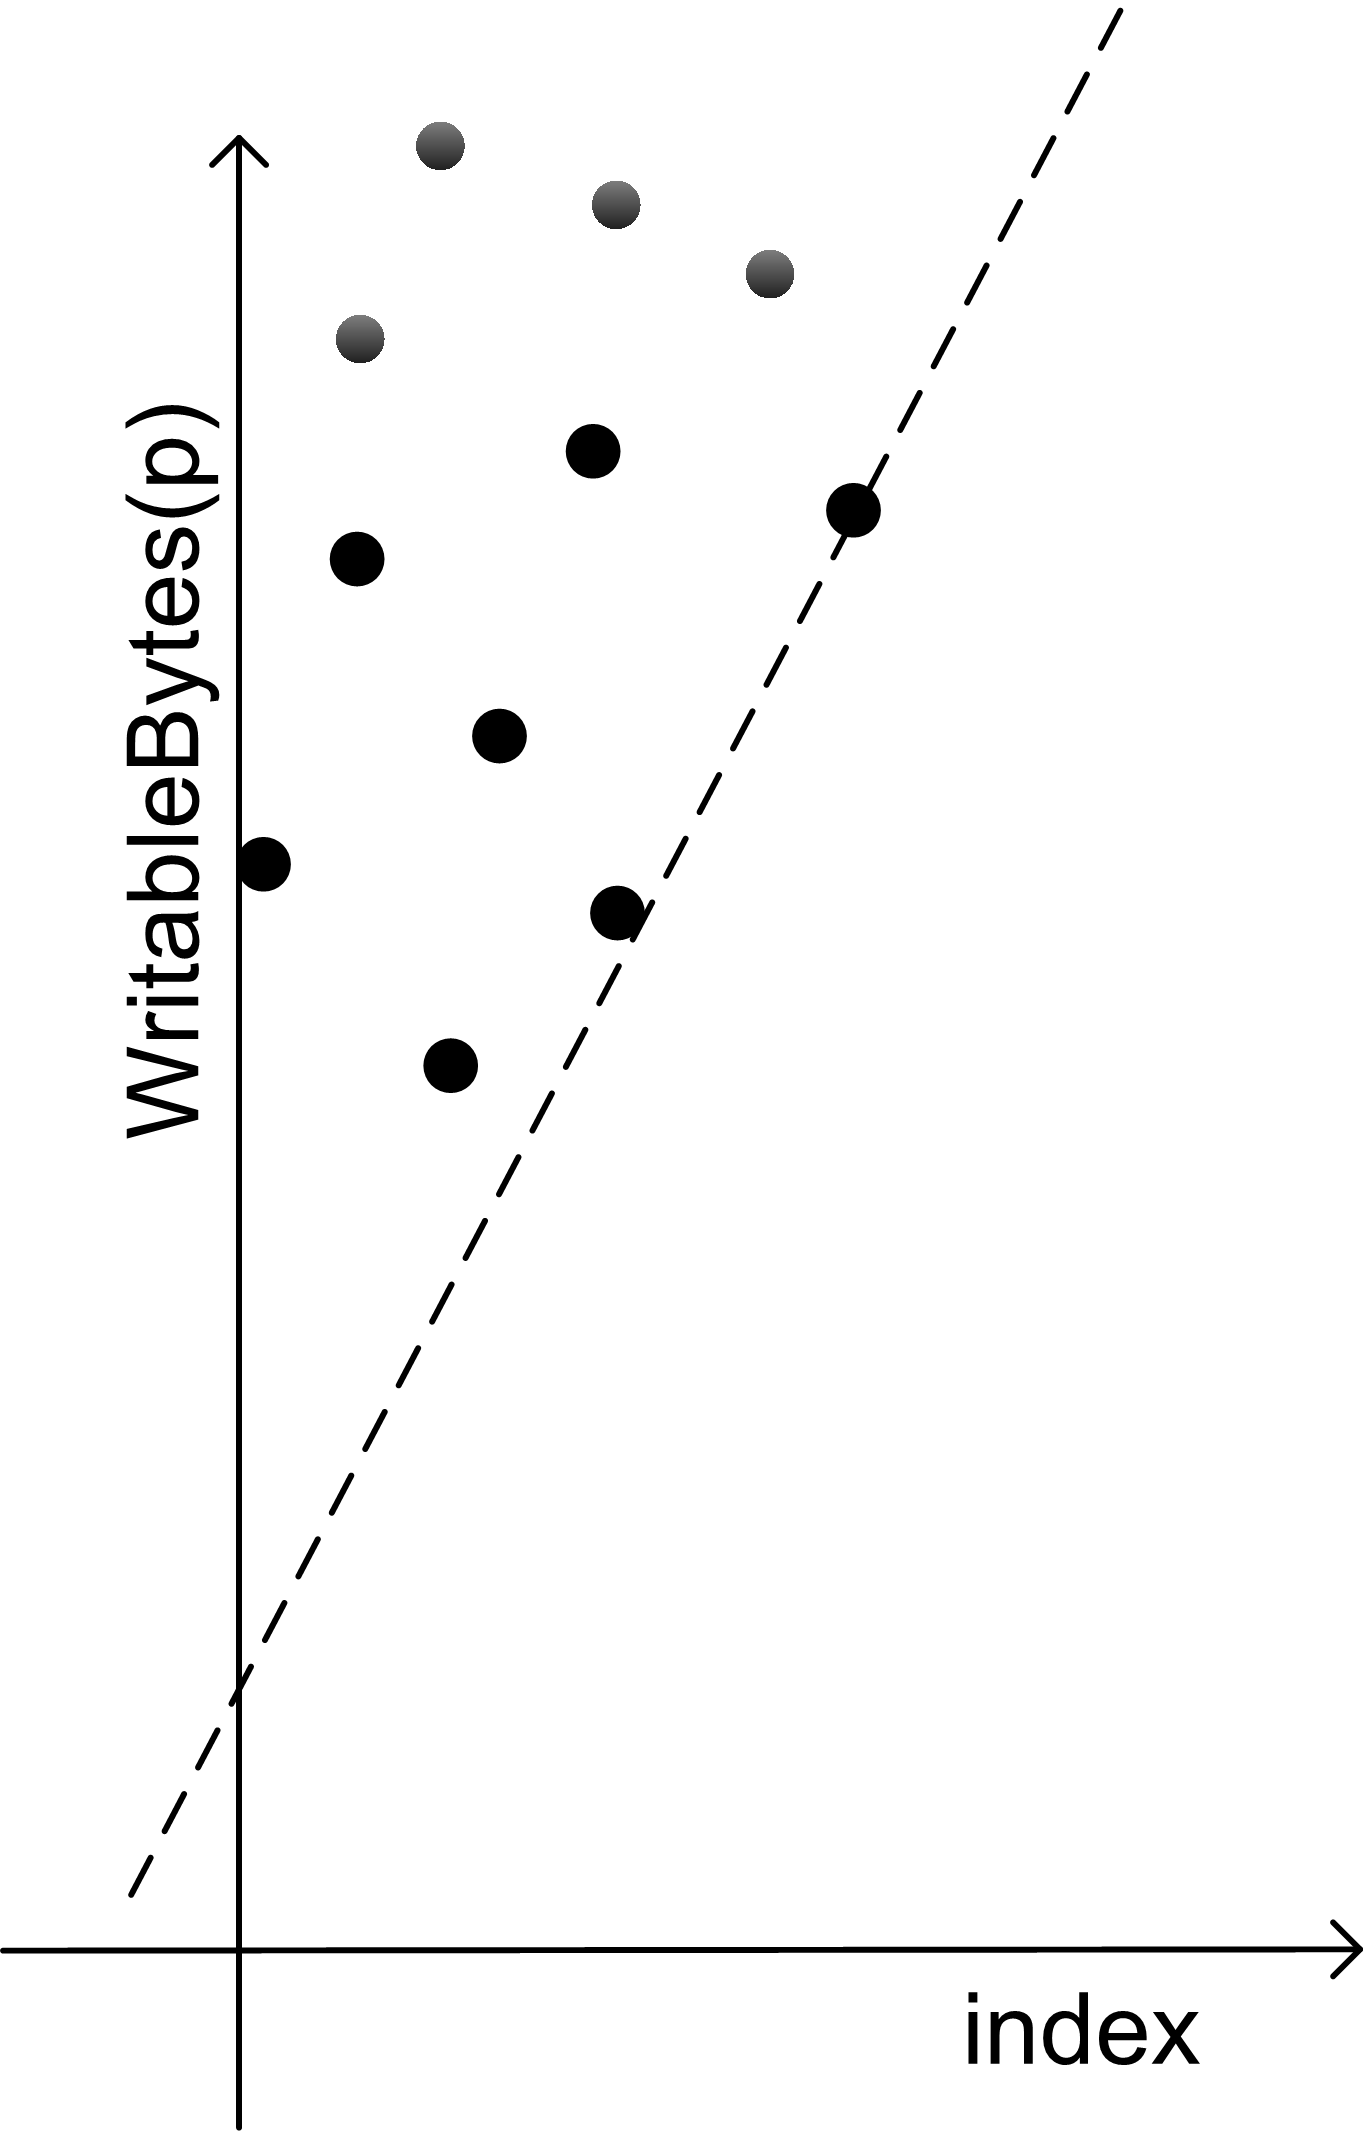
\includegraphics[scale=.57]{Concrete.png}
  \label{fig:concrete}
  }
  \subfigure[Intervals, \Order{n}]
   {
   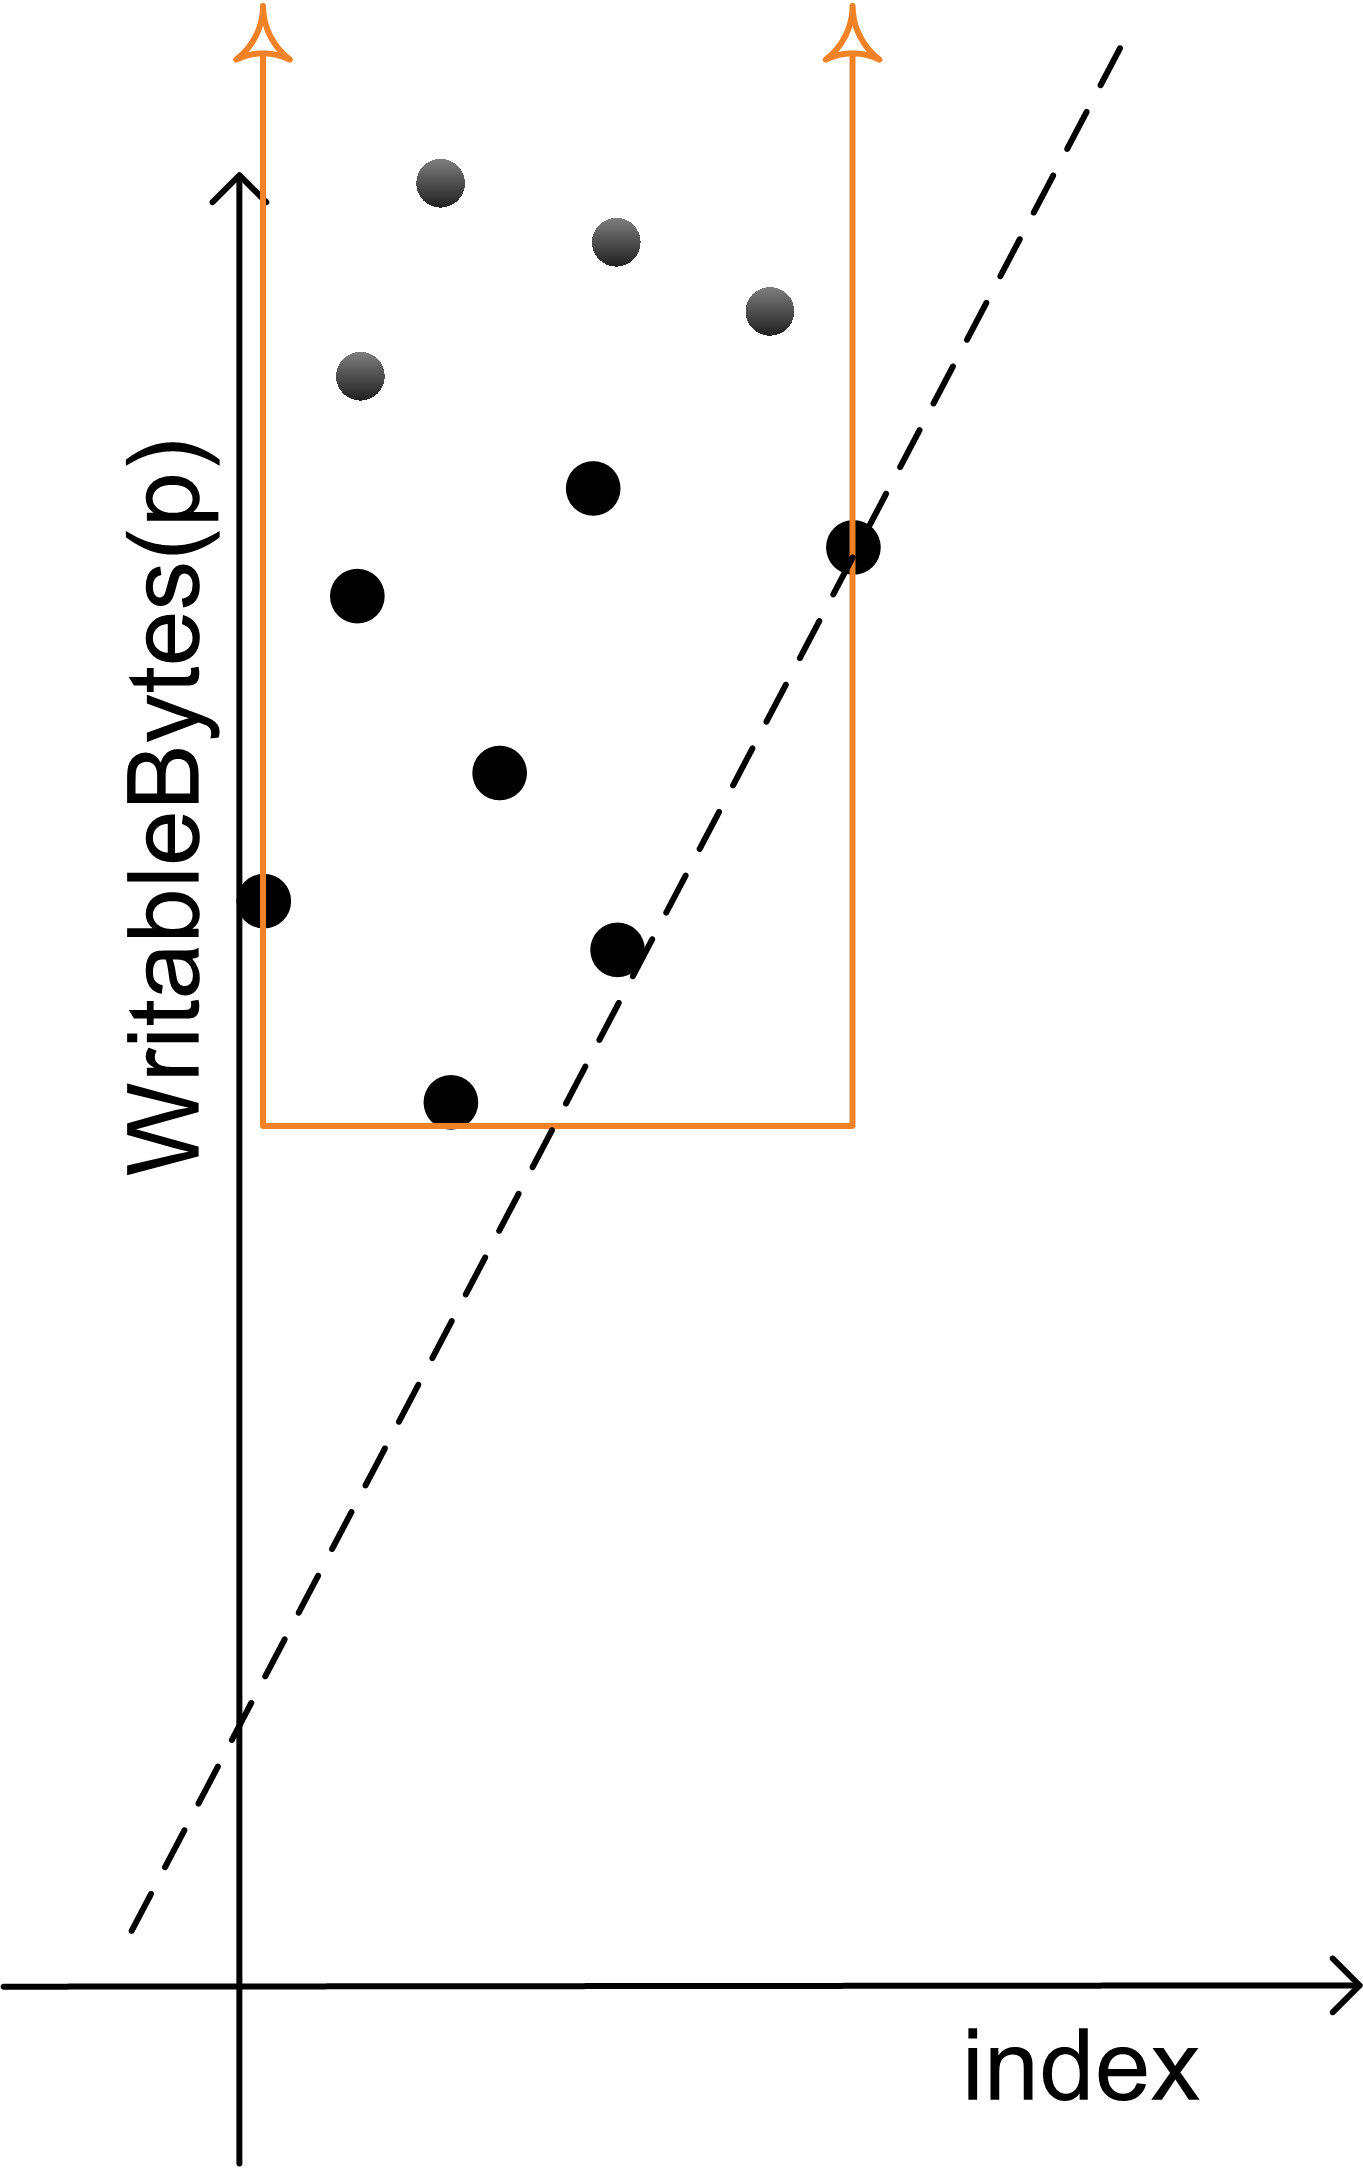
\includegraphics[scale=.57]{Intervals.png}
   \label{fig:intervals}
   }
   \subfigure[Octagons, \Order{n^3}]
   {
   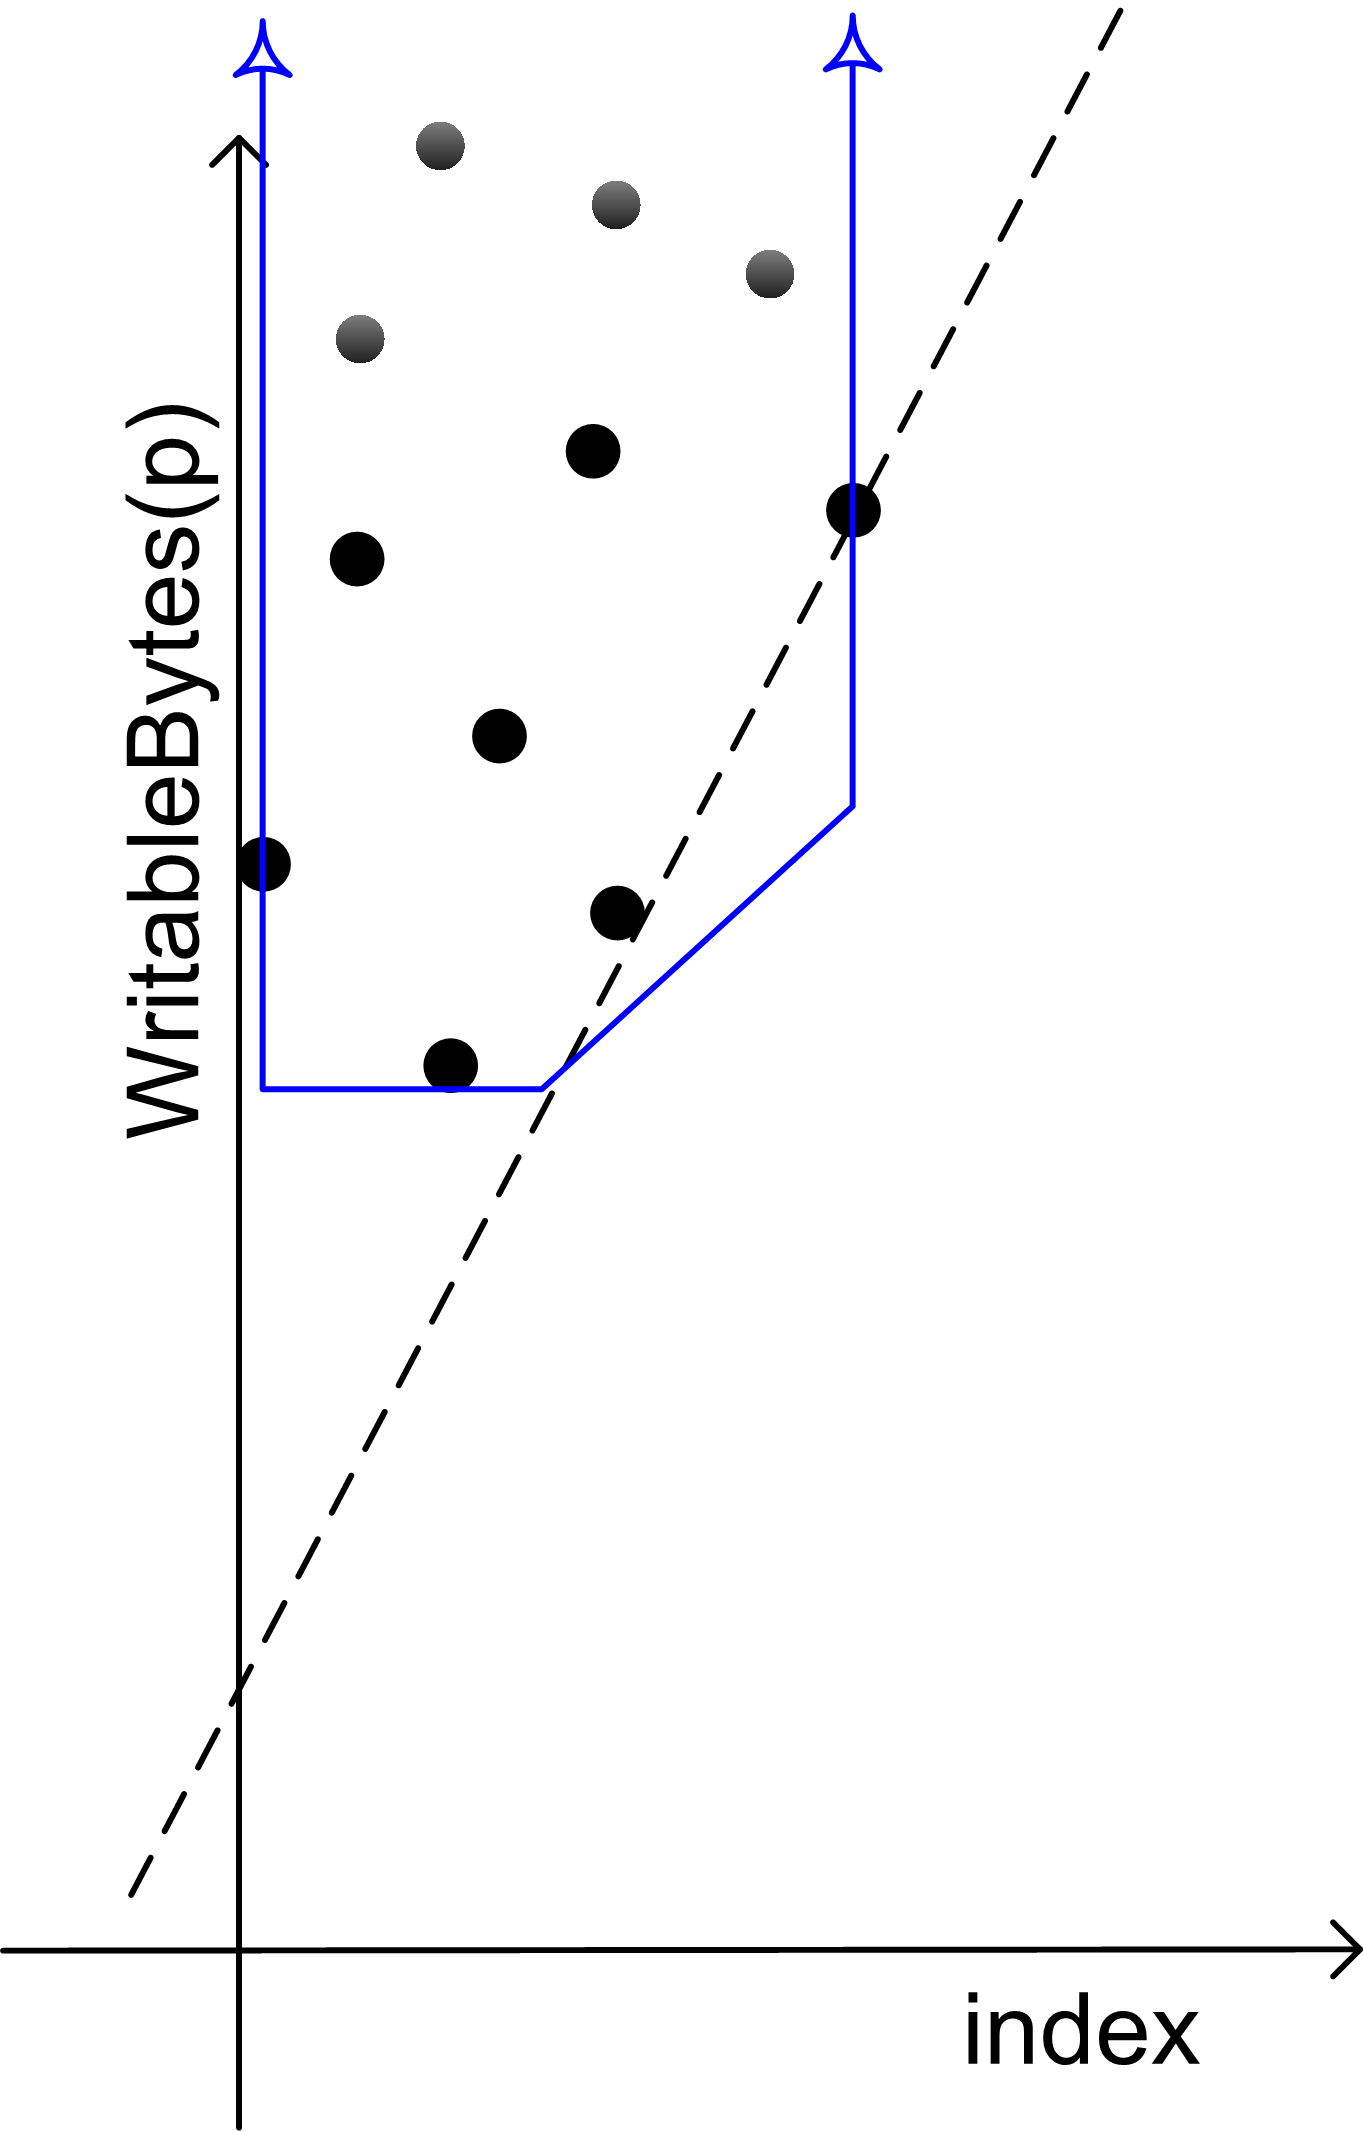
\includegraphics[scale=.57]{Octagons.png}
   \label{fig:octagons}
   }
   \subfigure[Polyhedra, \Order{2^n} in practice]
    {
    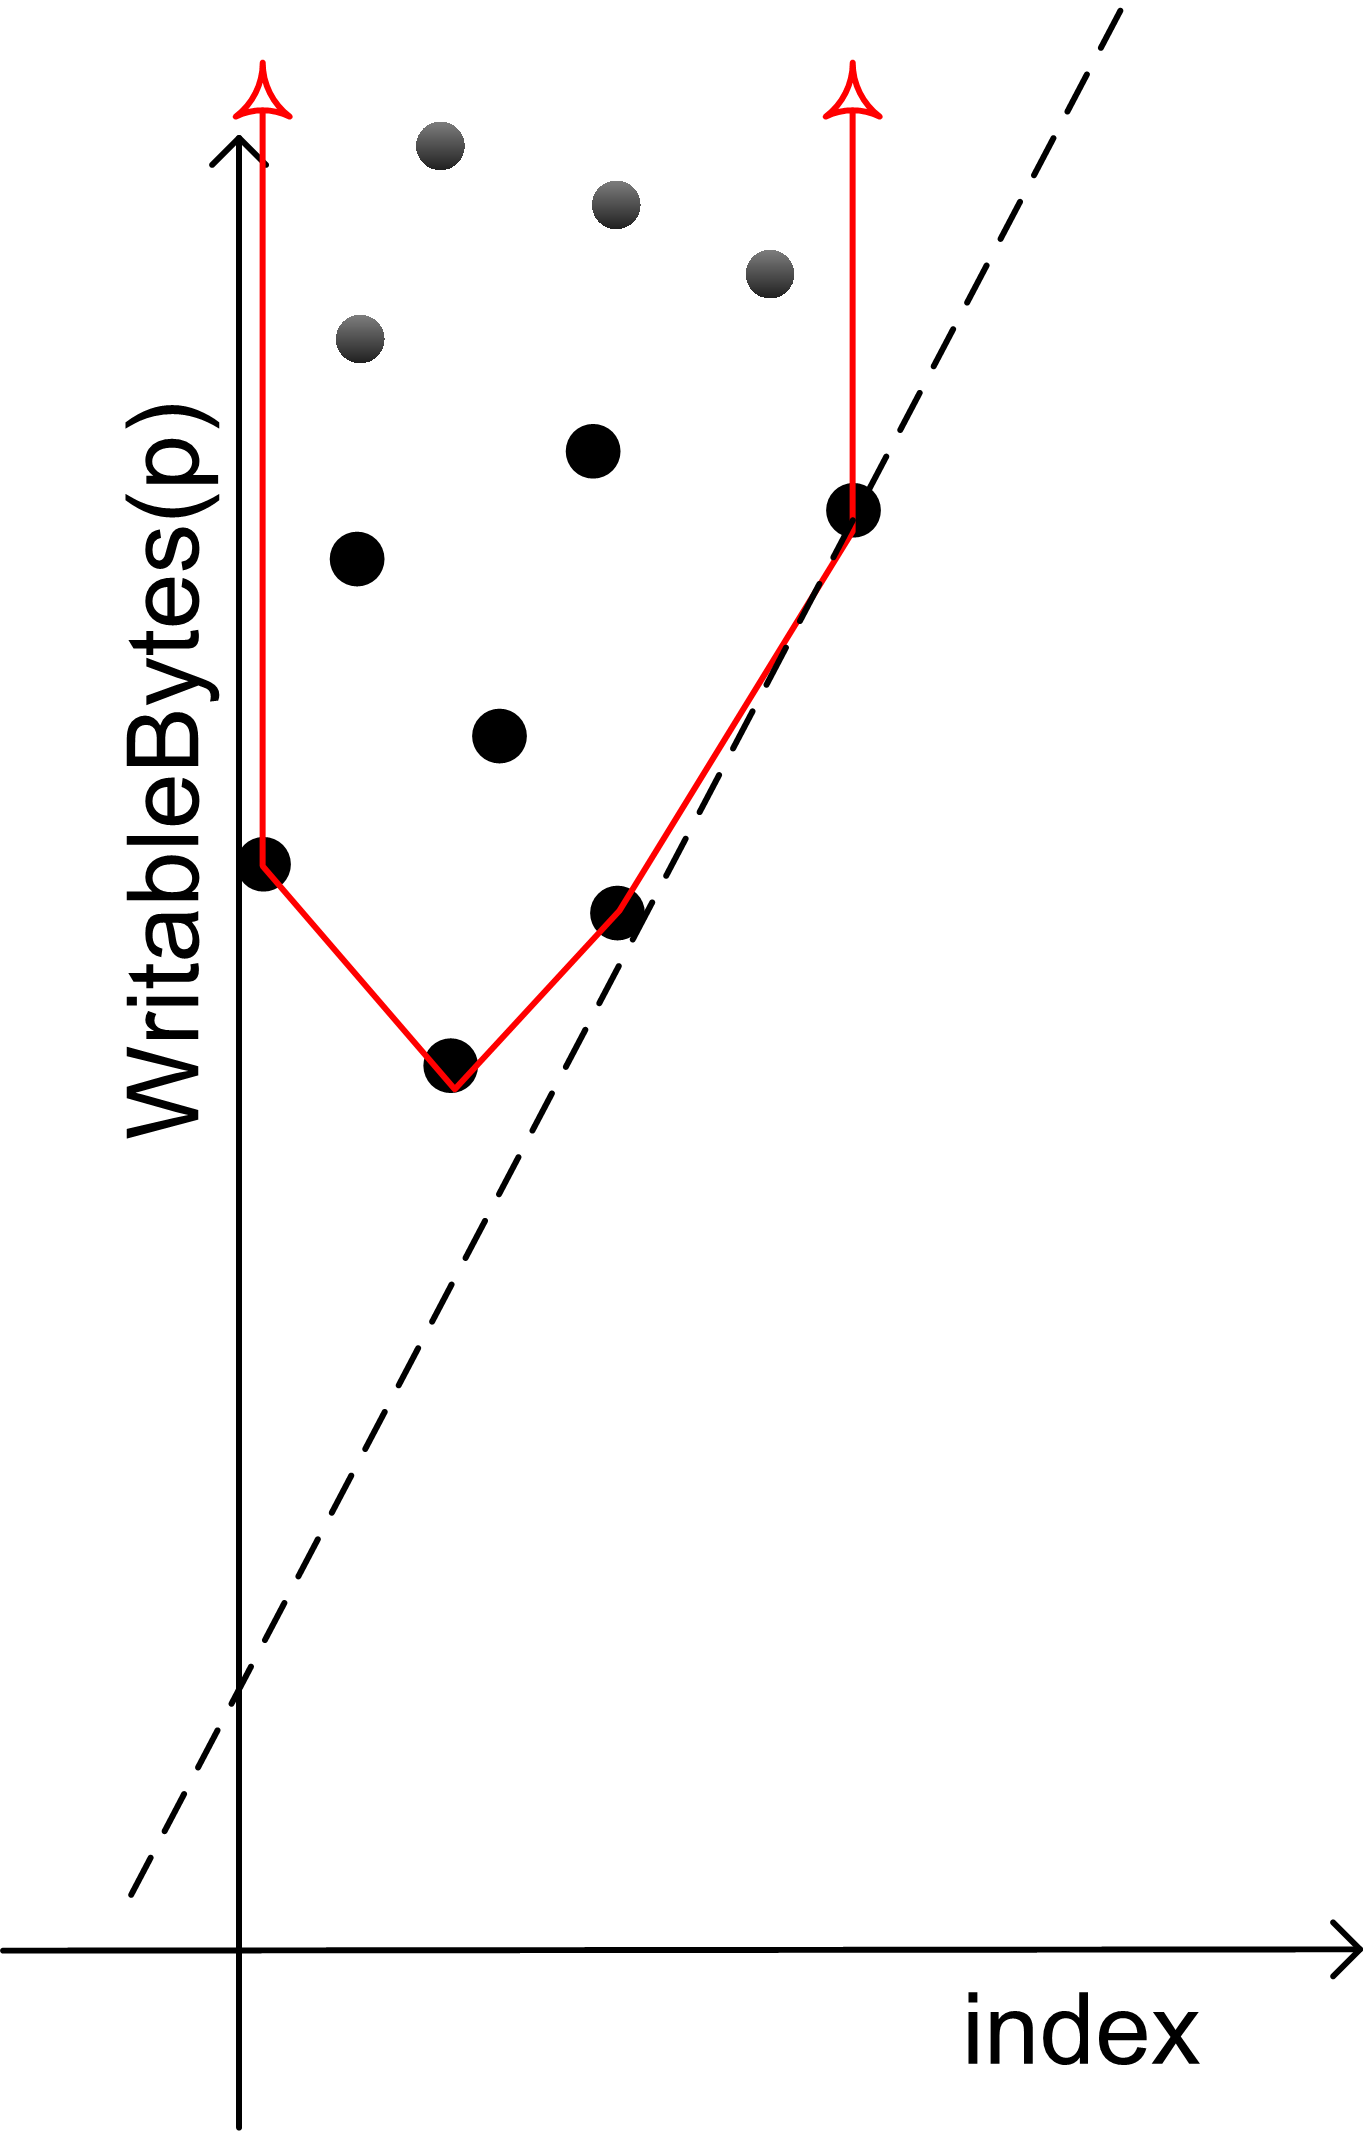
\includegraphics[scale=.57]{Polyhedra.png}
    \label{fig:polyhedra}
    }
   \subfigure[Stripes$\otimes$Intervals$\otimes$LinEq, \Order{n^3}, \Order{n} in practice]
   {
   \includegraphics[scale=.57]{stripes.png}
   \label{fig:stripes}
   }
\caption{The concrete points, and some approximations depending on the numerical abstract domain.
Intervals and Octagons are not precise enough to prove the property.
Polyhedra are precise, but also very expensive: they have an exponential complexity which shows up in practice.
The reduced product of Stripes$\otimes$Intervals$\otimes$LinEq represents a good trade off between precision and cost: the theoretical complexity is cubic, but in practice we experienced a linear behavior. 
}
\label{fig:exampleDomains}
\end{figure*}


The generic abstract semantics in Fig.~\ref{fig:AbstractSmallStepSemantics} can be instantiated with any numerical abstract domain containing the primitives $\mathsf{assign}$ and $\mathsf{check}$.
As a consequence the problem of checking the validity of memory accesses boils down to the problem of chosing the \emph{right} abstract domain. 

Existing numerical domains can be classified according to their precision/cost ratio.
The \emph{ideal} of a static analysis is to use the \emph{least} expensive domain which is precise \emph{enough} to prove the property of interests.

Let us consider the set of points \points\ of Fig.~\ref{fig:concrete}
corresponding to all the possible values that \WB{p} and \code{index}
assume at some memory access $\code{c = *(p + index)}$.
Geometrically, the memory access is safe as all the concrete values
are included in the upper-right quadrant delimeted by the lines
\code{index = 0} and \code{\WB{p} = base+index*sizeof(*p)}.  Proving it using an abstract domain
\adom{A} requires inferring an abstract element $\ael{a} \in \adom{A}$
such that $\points \subseteq \gamma(\ael{a}) \subseteq \plane$.

Fig.~\ref{fig:intervals} shows that \Intervals\ alone is not precise
enough for our purposes: the best approximation for \points\ with
\Intervals\ is not completely included in \plane.  Intuitively, this
is because \Intervals\ does not keep relational information, \eg, any
relation between \WB{p} and \code{index} is abstracted away.

Weakly-relational numerical abstract domains such as
Octagons~\cite{Mine01-2} or Pentagons~\cite{LogozzoMaf08} have been
introduced as lightweight solutions for \emph{array} bounds
checking\footnote{Octagons capture relations in the
form $\pm \code{x} \pm \code{y} \leq a$, and Pentagons in the form of
$a \leq \code{x} \leq b\ \wedge \code{x} < \code{y}$.}.
Fig.~\ref{fig:octagons} shows that Octagons are more precise than
\Intervals, but they are still not precise enough to validate memory
accesses due to the multiplicative factor \code{sizeof(*p)} which makes
the slopes in Fig.~\ref{fig:exampleDomains} possibly non-45$^\circ$.

Fig.~\ref{fig:polyhedra} shows that the convex hull
$\mathsf{CH}(\points)$ of the points \points\ is included in \plane.
The geometrical interpretation of the elements of the abstract domain
of Polyhedra (\Polyhedra)~\cite{CousotHalbwachs78} is exactly their
convex hull\footnote{Polyhedra capture arbitrary linear inequalities
among variables: $\Sigma_{i} a_i \cdot \code{x_i} \leq b$.}.  The main
drawback of using \Polyhedra\ is its worst case cost, which for the
most common operations is exponential in time and space (and this is a
lower-bound~\cite{KhachiyanBBEG06}).  In
Sect.~\ref{sec:Experiments} we will provide experimental evidence that 
that the worst case is attained in practice.

In \Clousot\ we are interested in the scalability of the analyses.
Therefore, we rejected the use of general purpose, precise but very
expensive abstract domains such as \Polyhedra.  Instead, we have
chosen a different path, which consists in (a) designing abstract
domains focused on a particular property; and (b) combining domains using
well-known techniques such as the reduced product.  For our analysis,
we designed a new numerical abstract domain, \Stripes, and we combined
it with \Intervals\ and \Karr\ to achieve precision without giving up
on performance.  Fig.~\ref{fig:stripes} illustrates the (best)
approximation for \points\ within the abstract domain $\Stripes
\otimes \Intervals \otimes \Karr$, which is included in \plane.

In the next sections we present the details of \Stripes, its reduction
with \Intervals\ and \Karr, and the results of our practical
experiments.



\section{The Stripes abstract domain}
We introduce a novel, weakly-relational domain Stripes, \Stripes,
focused on the inference and checking of (upper bounds on) memory
accesses that use a base, an index, and a multiplicative factor. 
We define the order, the join, the meet and the widening operators.

\subsection{Constraints}
As a first approximation, \Stripes\ captures constraints of the form 
$\WB{\var{p}}-\sizeof{T}*(\var{count}[+\var{base}])>\const{k}$ 
where $\WB{\var{p}}$, $\var{count}$, and optionally $\var{base}$ are variables, \code{T} is a type, and $\const{k}$ is an integer constant.
The intuition behind it is that the pointer $\var{p}$ is defined at least on $\var{count}[+\var{base}]$ elements of its type, and on $\const{k}$ additional bytes.

In  practice, these constraints are used in a more generic way: the
first element may be any variable (and not only the writable bytes of
a pointer) and the $\sizeof{T}$ may be any numerical value (and not
only the size of the type of the pointer target). 
Then the constraints captured by the Stripe domain are
$\var{z}-\const{k_1}*(\var{x}[+\var{y}])>\const{k_2}$.

\subsection{Abstract domain structure}

\subsubsection*{Abstract elements} 
We represent \Stripes\ elements as maps from variables to constraints.
We have chosen maps as they allow efficient manipulation of \emph{directional} constraints:
\[
\Stripes = \funzione{\variables_{\WBonly}}{\parti{(\variables_{\WBonly} \times (\variables_{\WBonly} \cup \bot) \times \naturalnumbers \times \naturalnumbers)}}.
\]
Intuitively, the domain of the map contains the variable $\var{z}$, the first and second component of the 4-tuple represent the two variables $\var{x}$ and $\var{y}$ ($\bot$ if it is not present), the third component is $\const{k_1}$ and the last one is $\const{k_2}$.\\

\paragraph{Example (Representation of stripes constraints)}
The two  constraints
$\var{z} - 4*\var{y} > 0$ and $\var{z} - 2*(\var{x}+\var{u}) \geq 5$ 
are represented in \Stripes\ by the map
$ \funzioneDue{\var{z}}{\{ (\var{y}, \bot, 4, 0), (\var{x}, \var{u}, 2, 4)\}} $. \qed


\subsubsection*{Order}
An abstract state $\abstrs{s}_1$ in \Stripes\ is more precise than  $\abstrs{s}_2$ iff for each constraint in $\abstrs{s}_2$, $\abstrs{s}_1$ contains a constraint such that
(a) the three variables and the integer constant $\const{k_1}$ are the same;
and (b) $\const{k_2}$ is less or equal than the $\const{k_2}$ of $\abstrs{s}_2$ since if $\var{x} > \var{y}$ and $\var{y} > \var{z}$ then $\var{x} > \var{z}$ by transitivity of $>$.
Formally:
\begin{multline*}
\abstrs{s}_1 \sqsubseteq \abstrs{s}_2 \Longleftrightarrow  \forall \var{z} \in \domain{\abstrs{s}_2}, \forall (\var{y}, \var{x}, k_1, k^2_2) \in \abstrs{s}_2(\var{z}).  \\
 \quad   \var{z} \in \domain{\abstrs{s}_1}\ \land \\
 \quad  \exists (\var{y}, \var{x}, k_1, k^1_2) \in \abstrs{s}_1(\var{z}). k^2_2 \leq k^1_2
\end{multline*}


\subsubsection*{Top and Bottom}
The largest element of \Stripes\ is a map with no information: $\lambda \code{z}.\ \emptyset$.
An abstract state $\ael{s}$ is bottom iff it contains a contradiction: \eg\ $[\code{z} \mapsto \{ (\code{y}, \bottom, 1, 0)\}, \code{y} \mapsto \{ \code{z}, \bottom, 1, 0)]$.

\subsubsection*{Join}
The upper bound operator (a) keeps the constraints that are defined in both  operands; (b)  takes the smallest lower bound $k_2$ if it is different in the two constraints since if $\var{exp} > a$,  $\var{exp} > b $ and $a \geq b$  then $\var{exp} > b$ is an upper bound for both constraints.
Formally:
\begin{multline*}
\abstrs{s}_1 \sqcup  \abstrs{s}_2  =  \lambda \var{z}. \{ (\var{y},\var{x},\const{k_1},\const{k_2}) \mid  (\var{y},\var{x},\const{k_1},\const{k^1_2}) \in \abstrs{s}_1(\var{z}), \\
\quad (\var{y},\var{x},\const{k_1},\const{k^2_2}) \in \abstrs{s}_2(\var{z}), \const{k_2} =\min(\const{k^1_2}, \const{k^2_2}) \}.
\end{multline*}


\subsubsection*{Meet}
The lower bound operator traces the constraints of both operands. 
If both contain a constraint with the same variables $\var{x}$, $\var{y}$, and $\var{z}$, and the same integer value $\const{k_1}$, the operator keeps the largest integer value for the numerical lower bound.
\[
\begin{array}{l@{}l}
\abstrs{s}_1 \sqcap \abstrs{s}_2 = & \lambda \var{z}.
\left\{
\begin{array}{l}
(\var{y},\var{x},\const{k}_1,\const{k}_2) \mid (\var{y},\var{x},\const{k}_1,\const{k^1_2}) \in \abstrs{s}_1(\var{z}),\\  
\phantom{(\var{y},\var{x},\const{k}_1,\const{k}_2) \mid \quad} (\var{y},\var{x},\const{k}_1,\const{k^2_2}) \in \abstrs{s}_2(\var{z}),\\
\phantom{(\var{y},\var{x},\const{k}_1,\const{k}_2) \mid \quad} \const{k}_2 = \max(\const{k^1_2}, \const{k^2_2})\\
\end{array}
\right\}
 \\
& \cup\\
\multicolumn{2}{@{\hspace*{35pt}}c}{
\lambda \var{z}. \left \{
\begin{array}{l}
   (\var{y},\var{x},\const{k}_1, \const{k}_2) \mid ((\var{y},\var{x},\const{k}_1, \const{k}_2) \in \abstrs{s}_1(\var{z}) \wedge\\
  \phantom{(\var{y},\var{x},\const{k}_1, \const{k}_2) \mid \vee}    (\var{y},\var{x},\const{k}_1, \_) \not\in \abstrs{s}_2(\var{z}))\\
  \phantom{(\var{y},\var{x},\const{k}_1, \const{k}_2) \mid}\vee ((\var{y},\var{x},\const{k}_1, \const{k}_2) \in \abstrs{s}_2(\var{z}) \wedge\\
  \phantom{(\var{y},\var{x},\const{k}_1, \const{k}_2) \mid \vee}    (\var{y},\var{x},\const{k}_1, \_) \not\in \abstrs{s}_1(\var{z}))
\end{array}
\right \}}
\end{array}
\]

\subsubsection*{Widening}
\Stripes\ does not satisfy the ACC condition.
As a consequence, we need to define a widening operator to ensure convergence.
Our widening simply drops the constraints that are not stable between two iterations:
\[
\abstrs{s}_1 \widening \abstrs{s}_2= \lambda \var{z}. \abstrs{s}_1(\var{z}) \cap \abstrs{s}_2(\var{z}).
\]

\subsubsection*{Concretization}
The concretization function $\gamma_\Stripes \in \funzione{\Stripes}{\parti{\Adomf}}$ returns all the possible states that satisfy the constraints represented by the abstract state:
\begin{multline*}
\gamma_{\Stripes} (\abstrs{s})= \{\abstrf{f} \mid \forall \var{z} \in \domain{\abstrs{s}} \forall (\var{y},\var{x},\const{k_1},\const{k_2}) \in \abstrs{s}(\var{z}).\\ \abstrf{f}(\var{z})-\const{k_1}*(\abstrf{f}(\var{y})+\abstrf{f}(\var{x}))>\const{k_2}\}.
\end{multline*}

It is immediate to see that $\gamma_\Stripes$ is monotonic, and furthermore that it is a complete $\cap$-morphism.
Therefore, as the composition of monotonic functions is monotonic, the following theorem stating that \Stripes\ is a sound approximation holds:

\paragraph{Theorem (Abstraction)}
$\gamma_\Stripes$ as defined above is a complete $\cap$-morphism.
\smallskip
Therefore, it exists an $\alpha_\Stripes$ such that $\tupla{\parti{\Adomf}, \subseteq}\galois{\alpha_\Stripes}{\gamma_\Stripes}\tupla{\Stripes, \aless}$
.
As a consequence, $\tupla{\parti{\Cdom}, \subseteq}$ $\galois{\alpha_\Stripes \circ \alpha}{\gamma \circ \gamma_\Stripes}$ $\tupla{\Stripes, \aless}  $.
\qed

\subsection{Refinement of the abstract state}\label{sec:refinement}
A state of the Stripe domain may be internally refined, by carefully propagating information between constraints.

\paragraph{Example (Refinement of constraints)}
Consider the two stripes constraints $\var{x}-2*(\var{y}+\var{u})>4$
and $\var{y}-\var{z}>0 $.
From the first constraint we derive: 
\[
\var{x}-2*(\var{y}+\var{u})>4 \Longleftrightarrow \var{x}-2*\var{u}-4>2*\var{y} \Longleftrightarrow \var{x}/2-\var{u}-2>\var{y}.
\]
From the second constraint we derive that $\var{y}>\var{z} \Longleftrightarrow \var{y} \geq \var{z}+1$. 
Combining the two, we derive a new  stripe constraint: $\var{x}/2-\var{u}-2>\var{z}+1 \Longleftrightarrow \var{x}-2*(\var{u}+\var{z})>6$. \qed

The  above example can be easily generalized:
\paragraph{Lemma (Saturation)}
\label{lemma:chiusura}
  If an abstract state contains the two constraints
  \[
  \begin{array}{l}
    \var{x}-\const{k_1}*(\var{y}[+\var{u}])>\const{k_2}\\
    \var{y}-1*\var{z}>\const{k_3}\\
  \end{array}
  \]
  then we can infer the constraint $\var{x}-\const{k_1}*(\var{z}[+\var{u}])>\const{k_2}+\const{k_1}*(\const{k_3}+1)$.
\qed


The refinement enabled by the lemma above is important in practice.
It allows adding new constraints to the abstract state, without requiring an expensive closure to propagate the information.
Of course, Lemma~\ref{lemma:chiusura} does not guarantee the completeness of the saturation, but it is sufficent for our purposes, as illustrated by the next example.

\paragraph{Example (Saturation)}
Let us consider the example in Fig.~\ref{fig:InitToZero}.
Inside the loop, we have the abstract state $\abstrs{s} = \{ \WB{\var{a}}-4*\var{len} > -1, \var{len}-\var{i} > 0 \}$ \footnote{To simplify the reading, we present a stripe abstract state as a set of constraints.}. 
We have to check whether $\WB{\var{a}}\geq 4*\var{i}+4$.
We cannot do it directly by inspecting $\abstrs{s}$ as there is no direct relation between $\WB{\var{a}}$ and $\var{i}$. 
Applying the refinement of Lemma~\ref{lemma:chiusura}, we infer the constraint $\WB{\var{a}}-4*\var{i}>3$ which suffices to  validate the access:  $\WB{\var{a}}-4*\var{i}>3  \Longleftrightarrow \WB{\var{a}}>4*\var{i}+3 \Longleftrightarrow \WB{\var{a}}\geq 4*\var{i}+4$ . \qed

In our implementation we perform this  refinement  only on-demand when we need to check the proof obligations.

\fcomment{
Consider the following code:
\begin{lstlisting}[frame=lines]
int * p;
int count;
... //WB(p)-4*count > -1
for(int i=0; i<count; i++)
	*(p+i)=0;
\end{lstlisting}

Inside the loop, we have the constraints $\WB{\var{p}}-4*\var{count} > -1, \var{count}-\var{i} > 0$, and we have to check if $\WB{\var{p}}\geq 4*\var{i}+4$. We cannot do it directly on the state, as we do not have any direct relation between $\WB{\var{p}}$ and $\var{i}$. Through the refinement just described we obtain the constraint $\WB{\var{p}}-4*\var{i}>3$ that validates the condition $\WB{\var{p}}\geq 4*\var{i}+4 \Rightarrow \WB{\var{p}}>4*\var{i}+3 \Rightarrow \WB{\var{p}}-4*\var{i}>3$.\\
This type of refinement (that theoretically is not the only one, but in the practice is the only one interesting) is performed only on-demand when we check if an expression, used to check if an accesses to memory respects the bounds, holds.
}
\subsection{Transfer functions}
\subsubsection*{Assignment}
When an expression is assigned to a variable, we first drop all the constants that are defined on the assigned variable, and then we add some inferred constraints.
Formally: 
\[
\begin{split}
\assign(\var{x}, \expr{exp}, \ael{s})= & \mathrm{let\ } \ael{s}' =  \dropfun{\var{x}}{\ael{s}} \\
  & \mathrm{in\ \ } \ael{s}' \cup \mathcal{C}(\code{x},\code{exp}, \ael{s}').
\end{split}
\]
where
\begin{multline*}
\dropfun{\var{x}}{\abstrs{s}}=\lambda \var{y}. \{(\var{z}, \var{u}, \const{k_1}, \const{k_2}) \mid   \var{y} \neq \var{x}, \\
(\var{z}, \var{u}, \const{k_1}, \const{k_2}) \in {\abstrs{s}}(\code{y})\Longrightarrow \var{z}\neq \var{x} \land\var{u} \neq \var{x}\};
\end{multline*}
and $\mathcal{C}$ infers new constraints from an assignment and an abstract state. 
Few  representative cases for $\mathcal{C}$ follow.
In our implementation we consider a richer structure of expressions and cases.
\[
\begin{array}{l@{}l}
  \mathcal{C}(\code{x}, \code{y}, \ael{s})=& \funzioneDue{\var{x}}{ \ael{s}(\code{y})} \cup \\ 
   & [\var{v_1} \mapsto \{(\var{x}, \var{v_2}, \const{k_1}, \const{k_2}) \mid (\var{y}, \var{v_2}, \const{k_1}, \const{k_2}) \in \abstrs{s}(\var{v_1})\}] \\
\multicolumn{2}{l}{\mathcal{C}(\code{x}, \code{u + v}, \ael{s})=}
\\
&[\var{v_1} \mapsto \{(\var{u}, \var{w}, \const{k_1}, \const{k_2}) \mid (\var{x}, \bot, \const{k_1}, \const{k_2}) \in \adom{s}(\var{v_1})\}] \\
& \dots 
\end{array}
\]

\subsubsection*{Abstract checking}
To check a boolean expression, we first try to normalize it into a form like $\var{x}-\const{k_1}*(\var{y}[+\var{z}])>\const{k_2}$, and then we check if the abstract state contains a constraint which implies it.
Formally:
\[
\begin{array}{l}
\mathsf{check} (\expr{exp}, \abstrs{s})=
\\
\mathrm{let} (\var{x}-\const{k_1}*(\var{y}+\var{z})>\const{k^1_2}, b) = \normalize{\expr{exp}} \\
\mathrm{in}
\\
\mathrm{\ \ if\ }(b \land  \exists (\var{y},\var{z},\const{k_1},\const{k^2_2}) \in \abstrs{s}(\var{x}). \const{k^1_2} \leq \const{k^2_2})\ \mathrm{then\ }  \true\ \mathrm{else\ } \top
\end{array}
\]
We skip the details of $\mathsf{normalize}$. 
Roughly, it applies basic arithmetic identities to rewrite the expression.
If it fails to put the expression into a stripe constraint form, it returns a boolean value signaling the failure.

\section{Refined Abstract Semantics}
% Problems
  % #1 : underflow accesses
  % #2 : Need for equalites
  % #3 : Null values 
% Solutions:
  % #1 : Use Intervals
  % #2 : Use Karr
  % #3 : Refine the join
% Discussion 
  % On the use of lightweight abstract domains

We  refine the information captured by the \Stripes\ domain with \Intervals\ and the \Karr\ domain. 
\Intervals\ is needed to check lower bounds of accesses.
\Karr\ is needed to track linear equalities, and in particular to handle the compilation schema for \code{fixed} in C\#.

\subsection{Checking lower bounds of accesses}
\Stripes\ allows representing just partial numerical bounds on variables.
In fact, when $k_1 = 0$, a stripe constraint boils down to a numerical lower bound: $\code{z} > k_2$.
Nevertheless, in general we need to track numerical upper bounds on variables: Those may appear in expressions that must be evaluated to check under-flow accesses.
We use \Intervals\ to track the numerical bounds on variables.

\paragraph{Example (Need for numerical bounds)}
Let us consider the following code snippet (``$\code{...}$'' denotes an arbitrary boolean expression):
\begin{lstlisting}[frame=lines]
int *p;
...
// suppose that WB(p) = 12, a = 5
if (...) {
  b = 3;
}
else {
  b = 4;
}
*(p + (a-b)) = 0; // (*)
\end{lstlisting}
If we track just lower bounds, at \code{(*)} we have $\code{a} > 4, \code{b} > 2$, so that we cannot prove the memory access correct.
If we track both numerical bounds, at \code{(*)} we have that $\code{a} = 5, \code{b} \in [3,4]$, so that $\code{b -a} \in [1,2]$ which suffices to prove the access correct. \qed


The numerical abstract domain for the analysis is the product domain
$\Intervals \otimes \Stripes$.  All the domain operations are lifted
pair-wise to the product domain.  Sometimes we may want to use the
information contained in \Intervals\ to refine the information in
\Stripes.  For instance, to improve the precision of the join
operator, as shown by the next example.

\paragraph{Example (Refinement of \Stripes\ with \Intervals)}
Consider the following piece of code:

\begin{lstlisting}[frame=lines]
int[] array;
...
// suppose that array.Length - count > 0
if (count == 0)
  array = new int[1];
else 
  /* do nothing */ ;
\end{lstlisting}
Using \emph{just} \Stripes, at the join point we cannot conclude that $\var{array.Length} - \var{count} > 0$: inside the conditional, \code{array} is assigned a new value, so that the entry constraint is dropped.

Using $\Intervals \otimes \Stripes$, the abstract state after array creation is $\ael{p}_1 = \tupla{\tupla{\code{count} \in [0,0],\allowbreak \code{array.Length}\in [1,1]}, \lambda \var{z}.\ \emptyset}$; the abstract state at the end of the false branch is $\ael{p}_2 = \tupla{\emptyset,  \funzioneDue{\var{array.Length}}{(\var{count}, 1, 0) }}$.
The join is $\tupla{\emptyset, \allowbreak \funzioneDue{\var{array.\allowbreak Length\allowbreak}}{(\var{count}, 1, 0) }}$, as the interval component of $\ael{p}_2$ implies that $\var{array.Length} - \var{count} > 0$.
\qed



\subsection{Compilation  of \code{fixed}}
When the C\# compiler compiles a \code{fixed} statement which assigns
an array \code{arr} of type $\code{T}[]$ to a pointer \code{p}, it
generates code to check whether the \code{arr} is \code{null} or if
its length is 0.  If it is the case, then it assigns \code{null} to
\code{p}.  Otherwise it assigns the address of the first element of
\code{arr} to \code{p}.  Fig.~\ref{fig:fixed} depicts this compilation
schema.

\begin{figure}[b]
\begin{lstlisting}
  if (arr == null)
    p = null;
  else if (arr.Length == 0)
    p = null;
  else 
    p = &arr[0];
\end{lstlisting}
\caption{The (schema of the) code generated by the C\# compiler for the statement $\code{fixed(T* p = arr) \dots }$ when \code{arr} is an array.}
\label{fig:fixed}
\end{figure}

%
%  Experiments
%
%  Here for placement reasons
%
\begin{table*}[t]
\centering
\small
\begin{tabular}{@{}l|r r r r @{\hspace{5mm}} r@{}}
 & & & \multicolumn{2}{c}{\textbf{\# Accesses}}& \\
\textbf{Assembly} & \textbf{\# Methods} & \hspace{0.5cm}\textbf{Time} & \textbf{Checked} & \textbf{Validated} & \textbf{\%}\\
\hline
\code{mscorlib.dll}                & 18 084 & 3m43s  & 3 069 & 1 835 & 59.79\\
\code{System.dll}                  & 13 776 & 3m18s  & 1 720 & 1 048 & 60.93\\
\code{System.Data.dll}             & 11 333 & 3m45s  &   138 &    59 & 42.75\\
\code{System.Design.dll}           & 11 419 & 2m42s  &    16 &    10 & 62.50\\
\code{System.Drawing.dll}          &  3 120 & 19s    &    48 &    29 & 60.42\\
\code{System.Web.dll}              & 22 076 & 3m19s  &    88 &    44 & 50.00\\
\code{System.Windows.Forms.dll}    & 23 180 & 4m31s  &   364 &   266 & 73.08\\
\code{System.XML.dll}              & 10 046 & 2m41s  &   772 &   311 & 40.28\\
\hline
\hspace{0.5cm} Average             &        &        &       &       & 57.96
\end{tabular}
\normalsize
\smallskip
\smallskip
  \caption{The results of our analysis tested on the \NET\ assemblies without using any contract. The average analysis time is of 12ms per method.}
  \label{tab:experiments}
\end{table*}

Without any refinement, the analysis performed by \Clousot\ cannot
capture that $\WB{\var{p}} = \sizeof{T}*\var{array.length}$.  Two main
reasons for that: (1) it is not possible to represent a constraint in
the form of $\code{x} - a * \code{y} = 0$ in $\Intervals \otimes
\Stripes$; (2) At the join point, a state where \var{p} is \code{null}
is merged with one where $\WB{\var{p}}=\sizeof{T}*\var{array.length}$.

For (1), we refine the abstract domain to use \Karr, to retain linear
equalities: the abstract domain used in the analysis becomes $\Karr
\otimes \Intervals \otimes \Stripes$.

For (2), if $\code{arr = null}$ or \code{arr.} \code{Length = 0}, then
$\code{0} = $ $ \sizeof{T}*$ \var{array.}\var{Length} $ = \WB{\var{p}}
$ trivially holds.  As we are performing an over-approximation of the
reachable states, we can safely add $\WB{\var{p}}
=\sizeof{T}*\var{array.length}$ to our abstract state.


\section{Experiments}
\label{sec:Experiments}
We have implemented the analysis for unsafe memory accesses using the
Stripes domain in \Clousot. 
We have extensively tested our analysis on all the libraries of the \Net\ framework. 
Our experiments were conducted on a 2.4Ghz Intel Core Duo laptop, with 4Gbytes of RAM, running Windows Vista (Windows processor score 5.3). 
The target assemblies are taken from the \code{\%WINDIR\%\backslash} \code{Microsoft\backslash} \code{Framework\backslash} \code{v2.0.50727} directory of the test laptop. 
No pre-processing, manipulation or filtering of the assemblies has been conducted.

A primary goal for \Clousot{} is its use at development time during
compilation or even within the integrated development environment.
Thus, the performance of the analysis is crucial. Our specialized
domains provide us with excellent performance as reported in Tab.~\ref{tab:experiments}. 



\mafcomment{Seems out of place:
\Clousot\ supports the entire set of \MSIL\ instructions, it performs intra-procedural analysis, and it uses contracts and inferred postconditions for inter-procedural analysis. 
When contracts are not available, it assumes the worst-case. 
This makes the analysis possibly imprecise, leading to false-positive warnings.
}

The analysis is fast: the average analysis time per method is $12$ms.
We validate on average $57.96\%$ of the
unsafe memory accesses. This may not seem high at first glance. However,
consider the burden of human code reviews for unsafe code which is
currently a necessary practice. Our analysis cuts down the work load
in half, focussing the reviews on accesses that seem non-obvious to
prove correct. Nevertheless, we feel that we can improve the precision
of the unsafe analysis in two ways: 
\begin{enumerate}
\item We intend to remove short-comings in the current
implementation of the domains, resulting in unnecessary precision loss
or inability to prove facts that are implied. We intend to improve the
domains as described e.g., in Section~\ref{sec:refinement}.

\item The code we analyzed does not contain contracts. This leads to
  loss of precision when the proof obligation required in one method
  is established by the caller of the method, or sometimes several
  call frames higher on the stack.
As a consequence, without
contracts on the intermediate methods \Clousot{} reports warnings on
those memory accesses.  
\end{enumerate}
We are actively working on adding contracts to
eventually validate all memory accesses.  Furthermore, to simplify 
checking of Windows API uses, we plan to write a tool to convert
SAL annotations~\cite{DasEtAl06} into \Foxtrot{} annotations.  In
Section~\ref{sec:case-study} we discuss the results of manually
inspecting the warnings for \code{System.Drawing.dll} and formulating
necessary contracts.
 
\subsection{Comparison with Polyhedra}
The main claim of our work is that specialized domains targetting a
particular set of proof-obligations are \emph{required} to make
such analyses practical. If we were able to use off-the-shelf solvers
for more powerful domains, such as Polyhedra, specialized domains
would not be necessary. We used our experience with the Polyhedra
implementation used to infer loop invariants in Boogie~\cite{Boogie}, 
to evaluate the cost of using Polyhedra for the analysis of unsafe
MSIL code. Although this implementation of Polyhedra is not as
optimized as for example~\cite{PPL}, it has been well debugged and in use
for a number of years. In our experiment, we replaced the
$\Stripes\otimes\Intervals\otimes \Karr$ domain in our analysis with
the Polyhedra domain implementation of Boogie and ran it on the two
largest libraries in \Net. The results are shown in
Table~\ref{tab:polyhedra-runs}.

\begin{table}
\centering
\small
\begin{tabular}{@{}l|r r r @{\hspace{5mm}} r@{}}
  & & \multicolumn{2}{c}{\textbf{\# Accesses}}& \\
\textbf{Assembly} & \hspace{0.5cm}\textbf{Time} & \textbf{Checked} & \textbf{Validated} & \textbf{\%}\\
\hline
\code{mscorlib.dll}                & 125m52s$^*$  & 3 070 & 1 610  & 52.46\\
\code{System.dll}                  & 257m27s$^*$  & 1 576 &  744  & 44.94\\
\end{tabular}
\normalsize
\smallskip
\smallskip
\caption{Unsafe code analysis using the Polyhedra domain}
\label{tab:polyhedra-runs}
\end{table}

As is apparent from the timings, the Polyhedra domain is orders of
magnitude slower than our implementation using \Stripes{}. In our
runs, we used a 2 minute timeout per method. The timeout was reached
23 times on \code{mscorlib.dll} and 13 times on \code{System.dll}.  In
all fairness, the Parma library~\cite{PPL} is likely to be much faster
than the implementation of Polyhedra we used. However, it is unlikely
to consistently improve the execution by two orders of magnitude and
it would still suffer from exponential behavior on some methods where
the 2 minute timeout was reached. When removing the timeout, one
method in \code{mscorlib.dll} took 49 minutes to reach a fixpoint
using Polyhedra.

\subsection{System.Drawing case study}
\label{sec:case-study}
We analyzed the 19 warnings in \code{System.Drawing.dll} to determine
what contracts need to be written to avoid them, or whether they
represent true vulnerabilities. 

First, we found the use of two helper methods that required
pre-conditions:
\begin{lstlisting}[frame=lines]
  short GetShort(byte* ptr) {
    Contract.Requires(Contract.WritableBytes(ptr) 
                      >= sizeof(short));
    ...

  int GetInt(byte* ptr) {
    Contract.Requires(Contract.WritableBytes(ptr)
                      >= sizeof(int));
    ...
\end{lstlisting}
These helper methods simply load 16 bits or 32 bits from the given
pointer location using little-endian encoding and avoiding unaligned
accesses.

With the pre-conditions written as above, \Clousot{} no longer reports 
warnings within these helper methods. Instead, it reports warnings at
26 call-sites to these methods. The remaining warnings are all located
within 5 distinct methods.
\begin{enumerate}
\item One method uses an unmanaged heap
allocation routine to obtain memory from the marshal heap. Writing an
appropriate post-condition for this allocator eliminates the warnings
in that method.
\begin{lstlisting}[frame=lines]
public static IntPtr AllocHGlobal(int cb) {
  Contract.Ensures(Contract.WritableBytes(
                    Contract.Result<IntPtr>()) == cb);
    ...
\end{lstlisting}

\item The next method we examined actually contained an error
  leading to buffer overruns on read accesses.

\item The third method uses a complicated invariant on a data
  structure that involves indexing using a product expression of two
  variables. Our domains cannot currently track such products (only
  variables multiplied with constants). However, the code appears to be
  safe.

\item The fourth method extracts a \code{byte[]} from an auxiliary
  data structure and indexes it assuming the array contains 1K
  elements. Examining the data structure and all its construction
  sites, we determined that it is built via marshalling from an unmanaged
  Windows API call and the marshal annotation specifies that the buffer is
  to be allocated with the fixed size of 1K. Although we can specify this
  size as an object invariant on the auxiliary structure leading to
  the removal of the warning by \Clousot{}, our tool
  chain does not yet understand the marshalling constraints
  establishing the invariant.

\item Finally, the last function containing most of the accesses and
  calls to the helper functions \code{GetShort} and \code{GetInt},
  whose pre-conditions must be validated, exposed a shortcoming in our
  implementation. Upon examination, we determined that the analyzer
  infers a sufficiently strong loop invariant which implies the safety
  of the memory accesses and
  pre-conditions. However, our implementation was not able to show
  this implication automatically. 
\end{enumerate}
With the above contracts and fixes, \Clousot{} would validate 3
additional methods, but report false warnings in one method due to an index
expression we cannot handle, and another false warning in a new method
due to the lack of support for marshal annotations.

\subsection{Summary}
Overall, the analysis is fast enough to use in integrated development
environments. It achieves a higher level of
automation and scalability than existing tools. In fact, we found that
the tool rarely fails to infer the necessary loop invariants to
validate the memory accesses. More often, it is the lack of contracts
that limits our modular intra-procedural analysis. The
use of contracts not only allows reducing the false positive rate, the
contracts furthermore serve as checked documentation on important
safety invariants. \Clousot{} can catch
code changes or additions that fail to live up to the existing
specifications and thereby provide excellent static regression
checking. 

\section{Related work}
In addition to the work cited in the introduction, we wish to place
our work in the context of the following other related work.

\subsubsection*{Bounds analysis for C}
Rinard and Rugina published a powerful analysis of C programs to
determine aliasing, bounds, and sharing of memory, enabling bounds
optimizations, and parallelization~\cite{rugina00,rinardrugina}. Their analysis
infers a set of polynomial bounds on variables that are solved using a
linear programming problem to minimize the spread of the bound. The
reported analysis times are fast (in the same range as ours), but they
only report results for small examples. Their technique based on
solving a linear programming problem is quite different from using
symbolic abstract domains, but equally promising. A benefit of their
approach is that it performs inter-procedural analysis by inferring
relations for function inputs and outputs using a bottom up call graph
approach. However, this is also a major drawback, as for strongly
connected components of functions (recursively calling each other),
their analysis needs to compute a fixpoint. It is well known that
call-graphs built for very large applications (in particular
object-oriented programs) are imprecise, leading to very large
components~\cite{onelevelflow}, making such an approach unlikely to scale.

Das et.~al.~describe buffer overflow checking and annotation inference
on large Microsoft C/C++ code bases~\cite{DasEtAl06}. Few details of
the used numerical domains are public, but from the paper it is
apparent that for precision, their analysis performs path splitting,
meaning it analyzes paths separately through a function whenever the
abstract state at join points disagrees. The Stripes domain described
in this paper and the associated transfer functions and join operations are
geared towards providing precision without path splitting (our
analyzer does not perform path splitting).

\subsubsection*{Analysis of JNI} 
A few analyses for Java handle programs using the Java Native
Interface (JNI) ~\cite{jni}.  Furr and Foster in \cite{FurrFoster06}
present a restricted form of dependent types used to infer and
type-check the types passed to foreign functions via the JNI.  Tan
\emph{et al.} proposed a mixed dynamic/static approach to guarantee
type safety in Java programs that interface with C.  We are not
interested in type safety: in unsafe C\#, type errors are less common
than with the JNI, since the unsafe context is integrated in C\#, so that
(a) the compiler can still perform most type checking and (b) types
do not need to be serialized as strings (the most common type error in
using the JNI). Instead our analysis focuses directly on memory usage
via pointers, whereas previous work did not.

\subsubsection*{Interoperability of languages}
Recent work focuses on language interoperability.  Tan and
Morrisett,~\cite{TanMorrisett07}, advocate an approach in which the
Java bytecode language is extended with a few instructions useful to
model C code.  Hirzel and Grimm,~\cite{HirzelGrimm07}, take an
alternative approach with Jeannie, which is a language which subsumes
Java and C, and the burden of creating the ``right'' JNI for
interfacing the two languages is left to the compiler.  Matthews
and Findler,~\cite{MatthewsFindler07}, give an operational semantics
for multi-language programs which uses contracts as glue for the
inter-operating languages.  The \MSIL\ instruction set is rich enough
to allow an agile compilation of several languages: our analysis,
working at the \MSIL\ level does not need to take into account
inter-operability issues.

\subsubsection*{Static analyzers}
ESC/Java 2~\cite{ESCJava2} and Spec\# ~\cite{specsharp} use automatic
theorem provers to check programs.  Automatic theorem provers provide
a strong engine for symbolic reasoning (\eg\ quantifiers handling).
The drawbacks are that: (a) they require the programmer to provide
loop invariants and (b) they present scalability problems.  Analysis
times close to the one we obtain in \Clousot\ on shipped code are well
beyond the state-of-the art in automatic theorem proving.


\section{Conclusions}
We presented a new static analysis for checking memory accesses in
unsafe code in \NET.  The core of the analysis is a new abstract
domain, \Stripes, which combined with \Intervals\ and
\Karr, allows the analysis to scale to hundreds of thousands of lines
of code.  We have proven the soundness of the approach by designing
the static analysis using stepwise abstraction of a concrete transition
semantics.


\bibliographystyle{plain}
%\bibliography{bib}
\begin{thebibliography}{10}

\bibitem{PPL}
R{.} Bagnara, P{.}M{.} Hill, and E{.} Zaffanella.
\newblock The {P}arma {P}olyhedra {L}ibrary.
\newblock \texttt{http://www.cs.unipr.it/ppl/}.

\bibitem{Boogie}
M{.} Barnett, B{.}-Y{.}~E{.} Chang, R{.} DeLine, B{.} Jacobs, and K.~R{.}~M.
  Leino.
\newblock Boogie: A modular reusable verifier for {O}bject-{O}riented programs.
\newblock In {\em FMCO'05}. Springer-Verlag, November 2005.

\bibitem{BarMafFerLog07}
M{.} Barnett, M{.} F\"ahndrich, and F{.} Logozzo.
\newblock {Foxtrot} and {Clousot}: {L}anguage {A}gnostic {D}ynamic and {S}tatic
  {C}ontract {C}hecking for \texttt{.Net}.
\newblock Technical Report MSR-TR-2008-105, Microsoft Research, Redmond, WA,
  August 2008.

\bibitem{specsharp}
M{.} Barnett, K{.}R{.}M{.} Leino, and W{.} Schulte.
\newblock The {S}pec\# programming system: An overview.
\newblock In {\em CASSIS 2004}, 2004.

\bibitem{VenetBrat05}
G{.}~P{.} Brat and A{.} Venet.
\newblock Precise and scalable static program analysis at {NASA}.
\newblock In {\em IEEE Aerospace Conference}. IEEE, 2005.

\bibitem{ESCJava2}
D{.}~R{.} Cok and J{.} Kiniry.
\newblock {ESC/Java} 2: Uniting {ESC/Java} and {JML}.
\newblock In {\em CASSIS 2004}, 2004.

\bibitem{Cousot98}
P{.} Cousot.
\newblock The calculational design of a generic abstract interpreter.
\newblock In {\em Calculational System Design}. NATO ASI Series F. IOS Press,
  Amsterdam, 1999.

\bibitem{CousotCousot77}
P{.} Cousot and R{.} Cousot.
\newblock Abstract interpretation: a unified lattice model for static analysis
  of programs by construction or approximation of fixpoints.
\newblock In {\em POPL'77}. ACM Press, January 1977.

\bibitem{CousotCousot79}
P{.} Cousot and R{.} Cousot.
\newblock Systematic design of program analysis frameworks.
\newblock In {\em POPL '79}, pages 269--282. ACM Press, January 1979.

\bibitem{CousotHalbwachs78}
P{.} Cousot and N{.} Halbwachs.
\newblock Automatic discovery of linear restraints among variables of a
  program.
\newblock In {\em POPL '78}. ACM Press, January 1978.

\bibitem{onelevelflow}
Manuvir Das.
\newblock Unification-based pointer analysis with directional assignments.
\newblock In {\em Proceedings of the {ACM} {SIGPLAN} 2000 Conference on
  Programming Language Design and Implementation ({PLDI}-00)}, pages 35--46.
  ACM, 2000.

\bibitem{Dor01}
N{.} Dor, M{.} Rodeh, and M{.} Sagiv.
\newblock Cleanness checking of string manipulations in {C} programs via
  integer analysis.
\newblock In {\em SAS'01}, LNCS. Springer-Verlag, June 2001.

\bibitem{Dor03}
N{.} Dor, M{.} Rodeh, and M{.} Sagiv.
\newblock {CSSV}: towards a realistic tool for statically detecting all buffer
  overflows in c.
\newblock In {\em PLDI'03}. ACM Press, 2003.

\bibitem{FurrFoster06}
M{.} Furr and J{.}~S{.} Foster.
\newblock Polymorphic type inference for the {JNI}.
\newblock In {\em ESOP'06}. Springer-Verlag, April 2006.

\bibitem{DasEtAl06}
B{.} Hackett, M{.} Das, D{.} Wang, and Z{.} Yang.
\newblock Modular checking for buffer overflows in the large.
\newblock In {\em ACM ICSE'06}. ACM Press, 2006.

\bibitem{HirzelGrimm07}
M{.} Hirzel and R{.} Grimm.
\newblock Jeannie: granting {Java} native interface developers their wishes.
\newblock In {\em OOPSLA'07}. ACM, October 2007.

\bibitem{HorspoolVitek92}
R{.}~N{.} Horspool and J{.} Vitek.
\newblock Static analysis of postscript code.
\newblock In {\em ICCL'92}. IEEE, 1992.

\bibitem{Karr76}
M{.} Karr.
\newblock On affine relationships among variables of a program.
\newblock {\em Acta Informatica}, 6(2):133--151, July 1976.

\bibitem{KhachiyanBBEG06}
L{.} Khachiyan, E{.} Boros, K{.} Borys, K{.}~M{.} Elbassioni, and M{.} Gurvich.
\newblock Generating all vertices of a polyhedron is hard.
\newblock In {\em ACM SODA'06}. ACM Press, 2006.

\bibitem{jni}
S{.} Liang.
\newblock {\em Java Native Interface: Programmer's Guide and Specification}.
\newblock Sun Microsystems, 2001.

\bibitem{Logozzo07}
F{.} Logozzo.
\newblock Cibai: An abstract interpretation-based static analyzer for modular
  analysis and verification of {Java} classes.
\newblock In {\em VMCAI'07}. Springer-Verlag, January 2007.

\bibitem{LogozzoMaf08-2}
F{.} Logozzo and M{.}~A{.} F\"ahndrich.
\newblock On the relative completeness of bytecode analysis versus source code
  analysis.
\newblock In {\em CC'08}, LNCS. Springer-Verlag, March 2008.

\bibitem{LogozzoMaf08}
F{.} Logozzo and M{.}~A{.} F\"ahndrich.
\newblock Pentagons: A weakly relational abstract domain for the efficient
  validation of array accesses.
\newblock In {\em ACM SAC'08 - OOPS}. ACM Press, March 2008.

\bibitem{MatthewsFindler07}
J{.} Matthews and R{.}~B{.} Findler.
\newblock Operational semantics for multi-language programs.
\newblock In {\em POPL'07}. ACM, January 2007.

\vfill\eject

\bibitem{meyer97}
B{.} Meyer.
\newblock {\em Object-Oriented Software Construction (2nd Edition)}.
\newblock Professional Technical Reference. Prentice Hall, 1997.

\bibitem{Mine01-2}
A{.} Min\'e.
\newblock The octagon abstract domain.
\newblock In {\em WCRE 2001}. IEEE Computer Society, October 2001.

\bibitem{MuellerOlmSeidl04}
M{.} M{\"u}ller-Olm and H{.} Seidl.
\newblock A note on karr's algorithm.
\newblock In Springer-Verlag, editor, {\em ICALP'04}, LNCS, 2004.

\bibitem{rugina00}
R.~Rugina and C.~R. Rinard.
\newblock Symbolic bounds analysis of pointers, array indices, and accessed
  memory regions.
\newblock In {\em Proceedings of the {ACM} {SIGPLAN} 2000 Conference on
  Programming Language Design and Implementation ({PLDI}-00)}, volume 35.5 of
  {\em ACM Sigplan Notices}, pages 182--195, N.Y., June ~18--21 2000. ACM
  Press.

\bibitem{rinardrugina}
R.~Rugina and M.~C. Rinard.
\newblock Symbolic bounds analysis of pointers, array indices, and accessed
  memory regions.
\newblock {\em ACM Transactions on Programming Languages and Systems},
  27(2):185--235, 2005.

\bibitem{Schmidt08}
D{.}~A{.} Schmidt.
\newblock The internal and external logic of abstract interpretations.
\newblock In {\em VMCAI'08}. Springer-Verlag, January 2008.

\bibitem{SimonKing02-1}
A{.} Simon and A{.} King.
\newblock Analyzing string buffers in c.
\newblock In {\em AMAST'02}, LNCS. Springer-Verlag, September 2002.

\bibitem{SimonKing02-2}
A{.} Simon, A{.} King, and J{.} Howe.
\newblock Two variables per linear inequality as an abstract domain.
\newblock In {\em LOPSTR'02}, LNCS. Springer-Verlag, September 2002.

\bibitem{TanMorrisett07}
G{.} Tan and G{.} Morrisett.
\newblock Ilea: inter-language analysis across java and c.
\newblock In {\em OOPSLA'07}. ACM, October 2007.

\bibitem{Wagner00}
D{.} Wagner, J{.}~S{.} Foster, E{.}~A{.} Brewer, and A{.} Aiken.
\newblock A first step towards automated detection of buffer overrun
  vulnerabilities.
\newblock In {\em NDSS'00}, 2000.

\end{thebibliography}



\end{document}

 
